\section{Introduction}

Aeolian sediment transport is influenced by a variety of bed surface
properties that are commonly found in coastal environments, like:
moisture, shells, strandlines, salt crusts, bed slopes, vegetation,
non-erodible elements and antropogenic disturbances. The bed surface
properties influence aeolian sediment transport by changing the
sediment transport capacity and/or the sediment availability
\citep{Kocurek1999}. In current aeolian sediment transport models the
effects on the sediment transport capacity and sediment availability
are generally incorporated through a single parameter: the velocity
threshold. This approach appears to be a critical limitation in
existing aeolian sediment transport models for simulation of
real-world cases with spatiotemporal variations in bed surface
properties.

The velocity threshold was introduced by \citet{Bagnold1935}, and
incorporated in his initial aeolian sediment transport model
\citep{Bagnold1937a} according to:

\begin{equation}
  \label{eq:bagnold}
  \underbrace{
    \vphantom{
      C \frac{\rho_{\mathrm{a}}}{g} \sqrt{\frac{d_{\mathrm{n}}}{D_{\mathrm{n}}}}
    }
    q_{\mathrm{sat}}
  }_{
    \text{
      \parbox{5.5em}{
        \linespread{.5} \selectfont \centering
        sediment transport capacity
      }
    }
  }
  = \alpha 
  \underbrace{
    C \frac{\rho_{\mathrm{a}}}{g} \sqrt{\frac{d_{\mathrm{n}}}{D_{\mathrm{n}}}}
  }_{
    \text{
      \parbox{5.5em}{
        \linespread{.5} \selectfont \centering
        properties of sediment in transport
      }
    }
  }
  \left ( u_z - u_{\mathrm{th}} \right )^3
\end{equation}

\noindent in which $q_{\mathrm{sat}}$ [kg/m/s] is the equilibrium or
saturated sediment transport rate and represents the sediment
transport capacity. $u_z$ [m/s] is the wind velocity at height $z$ [m]
and $u_{\mathrm{th}}$ the velocity threshold [m/s]. The properties of
the sediment in transport are represented by a series of parameters:
$C$ [--] is a parameter to account for the grain size distribution
width, $\rho_{\mathrm{a}}$ [$\mathrm{kg/m^3}$] is the density of the
air, $g$ [$\mathrm{m/s^2}$] is the gravitational constant,
$d_{\mathrm{n}}$ [m] is the nominal grain size and $D_{\mathrm{n}}$
[m] is a reference grain size. $\alpha$ is a constant to account for
the conversion of the measured wind velocity to the near-bed shear
velocity following Prandtl-Von K{\'a}rm{\'a}n's Law of the Wall:
$\left(\frac{\kappa}{\ln z / z'} \right)^3$ in which $z'$ [m] is the
height at which the idealized velocity profile reaches zero and
$\kappa$ [-] is the Von K{\'a}rm{\'a}n constant. Many studies
following the work of \citet{Bagnold1937a} effectively proposed
different parameterizations for sediment properties
\citep[e.g.][]{Owen1964, Hsu1971, Sorensen2004} or changed the weight
of the velocity threshold \citep[e.g.][]{Kawamura1951,
  Lettau1978}. However, the characteristic structure and application
of these models stayed essentially the same.

\citet{Sherman1998} and \citet{Sherman2012} summarized the performance
of eight aeolian sediment transport models compared to field
measurements on a sandy beach. All the models systematically
overpredict the measured aeolian sediment transport rates, which is in
agreement with other coastal field studies \citep[e.g.][]{Jackson1999,
  Lynch2008, DavidsonArnott2009, Aagaard2014}. Besides, the original
model of \citet{Bagnold1937a} appeared to outperform the models of
later date. In an attempt to explain the poor performance of aeolian
sediment transport models in coastal environments, many authors
emphasized the importance of bed surface properties. Typical bed
surface properties that are found along the coast and assumed to
explain at least partially the poor performance of aeolian sediment
transport models are high moisture contents \citep[e.g.][]{Wiggs2004,
  DavidsonArnott2008, Darke2008, McKennaNeuman2008, Udo2008,
  Bauer2009, Edwards2009, Namikas2010, Scheidt2010}, salt crusts
\citep[e.g.][]{Nickling1981}, bed slopes \citep[e.g.][]{Iversen2006},
vegetation \citep[e.g.][]{Arens1996, Lancaster1998, Okin2008, Li2013,
  Dupont2014}, shell pavements \citep[e.g.][]{VanDerWal1998,
  McKennaNeuman2012} and sorted and armored beach surfaces
\citep[e.g.][]{Gillette1989, Gillies2006, Tan2013, Cheng2015}. The
influence of these bed surface properties on aeolian sediment
transport has been investigated and often resulted in modified values
for the velocity threshold \citep[e.g.][]{Howard1977, Dyer1986,
  Belly1964, Johnson1965, Hotta1984, Nickling1981, Arens1996,
  King2005}.

A critical limitation of the use of the velocity threshold alone to
cope with the influence of bed surface properties is that it changes
inherently in time and space \citep{Stout2004} and that it accounts
for two fundamentally different phenomena:
\begin{enumerate}
\item The change in the sediment transport capacity which represents
  the ease of sediment transport \emph{over} a given bed; and
\item The change in sediment availability, which represents the ease
  of sediment entrainment \emph{from} a given bed.
\end{enumerate}
\noindent Although in uniform and constant situations, like often used
in wind tunnel experiments, the difference might be negligible, in
real-world field conditions it is not. The difference is most apparent
when observing transport over a bed with spatial variations in bed
surface properties. For example due to tidal motions in the intertidal
beach area, emergence of roughness elements in the dry beach area and
vegetation in the dune area. In addition, temporal variations in bed
surface properties, for example due to tidal spring/neap cycles, rain
showers, storm surges, seasonal variations in vegetation and
progressive armoring of the beach, increase the need for simulation
rather than parameterization of bed surface properties and sediment
availability (as discussed in section \ref{sec:challenges}).

This paper presents a new model approach for aeolian sediment
transport. The model simulates rather than parameterizes bed surface
properties and sediment availability. The model explicitly defines
sediment availability following \citet{deVries2014a} and introduces
multi-fraction aeolian sediment transport in order to simulate
processes that limit the availability of sediment, like beach
armoring, and processes that enhance the availability of sediment,
like hydraulic mixing. Consequently, the model can cope with arbitrary
spatiotemporal configurations of bed surface properties. Although
validation of the model is ongoing, the performance of the model is
illustrated using four prototype cases, the simulation of two wind
tunnel experiments from literature \citep{Nickling1995, Dong2004b} and
a sensitivity analysis of newly introduced parameters.

\vspace{.5cm}

In literature the \emph{velocity threshold} is used interchangeably to
describe the (change in) sediment transport capacity and sediment
availability. In this paper the term \emph{velocity threshold} is
strictly used to describe the (change in) sediment transport capacity
(Equation \ref{eq:bagnold}). The term \emph{sediment availability} is
used in accordance with the terminology proposed by
\citet{Kocurek1999}, which is often referred to as \emph{sediment
  supply} in literature.

\section{Model Challenges: Bed Surface Properties} \label{sec:challenges}

The importance of spatiotemporal variations in bed surface properties
for aeolian sediment transport is most apparent when observing
transport over a bed consisting of both erodible and non-erodible
fractions. Many studies have investigated the influence of varying
grain sizes on aeolian sediment transport. In most cases it involved
studies on the influence of non-erodible or roughness elements using
either field experiments \citep[e.g.][]{DavidsonArnott1997,
  Gillies2006, Tan2013} or wind tunnel experiments
\citep[e.g.][]{Gillette1989, Nickling1995, McKennaNeuman1995,
  Dong2004b, McKennaNeuman2012} and occasionally numerical modeling
\citep[e.g.][]{Turpin2010}. The studies typically use granular
material with a clear bi-modal distribution. A flat sandy surface is
then partially covered by a significantly larger grain size fraction
ranging from shells and gravel to pebbles and cobbles. Typically the
coverage of non-erodible elements is expressed using the roughness
density $\lambda$ as described by
\citet{Raupach1993}. \citet{Raupach1993} uses the roughness density to
determine the relative increase in the shear velocity threshold
according to:

\begin{equation} \label{eq:raupach}
R_{\mathrm{t}} = \frac{u_{\mathrm{* th, S}}}{u_{\mathrm{* th, R}}} = \frac{1}{\sqrt{(1 - m \sigma \lambda) (1 + m \beta \lambda)}}
\end{equation}

\noindent in which $u_{\mathrm{* th, S}}$ is the shear velocity
threshold with a bare surface, $u_{\mathrm{* th, R}}$ is the shear
velocity threshold with a surface including non-erodible elements and
$m$, $\sigma$ and $\beta$ are calibration coefficients that account
for the size and shape of the non-erodible elements. \mrq{3.2}

\subsection{Temporal Variations in Bed Surface Properties}

The concept of the roughness density is useful to describe the
instantaneous influence of roughness elements in the bed on aeolian
sediment transport. However, it does not account for the fact that
roughness elements tend to emerge from the bed over time due to
winnowing of fines. Following \citet{Gillette1989},
\citet{Nickling1995} and \citet{McKennaNeuman1995} showed that the
winnowing of fines and the emergence of roughness elements result in a
time-dependent aeolian sediment transport rate. The time-dependency is
caused by a recurrence relation between sediment transport and
sediment availability. Consequently, neither the roughness density nor
the sediment availability can be determined a-priori. We argue that
process-based simulation of bed surface properties rather than
parameterization is needed to solve the instantaneous sediment
availability.

\citet{McKennaNeuman2012} shows that even small shell fragments cause
a sandy surface to be armored over time. But even in the absence of
non-erodible roughness elements, spatiotemporal variations in bed
surface properties may develop as the transport capacity is inversely
related to the grain size \citep{Bagnold1937a} resulting in sediment
sorting: a coarsening of the bed surface and downwind deposition of
fines \citep{Bagnold1937a, VanDerWal2000, Arens2002}.

\subsection{Spatial Variations in Bed Surface Properties}

Spatial variations in bed surface properties occur naturally in
coastal environments. For example, strandlines locally cover the
erodible bed and reduce the sediment availability. However,
strandlines not necessarily reduce the sediment transport capacity to
the same extent and may even increase the transport capacity due to
fully elastic collisions with the sediment in transport. The
distinction between sediment availability and sediment transport
capacity in relation to bed surface properties is not offered by
existing models.

\citet{Dong2004b} describes a similar situation in a wind tunnel. In
their experiment a patch of gravel (10 - 40 mm) is positioned downwind
of a patch of sandy material. \citet{Dong2004b} show how the gravel
patch reduces the aeolian sediment transport rate downwind of the
domain compared to the situation without the gravel. However, in all
conditions sediment passes the patch, while sediment availability from
the patch is zero. There seems to be a tendency of an increase in
sediment transport rate with increasing patch size when the patch size
is relatively small. This is attributed to the change in transport
characteristics due to fully elastic collisions between the sand
grains and the gravel. Consequently, the saltation height and rebound
angle increase and in turn influence the sediment transport
capacity. Only for large patch sizes the trapping of sand grains in
the gravel pores becomes a dominant process resulting in a decrease in
the sediment transport rate downwind of the gravel patch.

\citet{Dong2004b} acknowledged the limitations of the use of the shear
velocity threshold to describe the results of his wind tunnel
experiments. Therefore they introduced a factor in the aeolian
sediment transport formulation of \citet{Dymin1954}
%\citet[][quoted by \citet{Greeley1985}]{Dymin1954}
that depends on the length of the
gravel patch squared. Although an important observation, the method is
hardly generalizable to more realistic situations where moist
intertidal beaches are located adjacent to strandlines and armored
beaches that subsequently border a vegetated dune. Therefore, to cope
with spatially varying bed surface properties an aeolian sediment
transport model is needed that provides a generic distinction between
the effect of bed surface properties on the sediment transport
capacity and sediment availability.

\section{Model Concepts: Sediment Availability, Saturated Transport
  and Entrainment}
\label{sec:model_concepts}

The sediment transport capacity and sediment availability together
determine the sediment entrainment. Sediment availability differs from
entrainment in that the availability defines the \emph{potential}
erosion of the bed, while the entrainment defines the \emph{actual}
erosion of the bed. If aeolian sediment transport is
transport-limited, the sediment availability is larger than
entrainment and not all available sediment will be
transported. Consequently, entrainment is governed by the sediment
transport capacity. If aeolian sediment transport is
availability-limited, entrainment is equal to the sediment
availability. Whether aeolian sediment transport is transport- or
availability-limited depends on the balance between the sediment
transport capacity and the sediment availability that are both
influenced by bed surface properties. In the literature various
concepts to incorporate the influence of bed surface properties in
aeolian sediment transport models can be found: \mrq[m]{3.1}

\begin{enumerate}
\item the concept of the shear velocity threshold
  \citep[e.g.][]{Howard1977, Dyer1986, Belly1964, Johnson1965,
    Hotta1984, Nickling1981, Arens1996};
\item the concept of critical fetch \citep[e.g.][]{Bauer2002,
    DelgadoFernandez2010};
\item the concept of explicit availability \citep[or
  supply;][]{deVries2014a}.
\end{enumerate}

From these concepts the shear velocity threshold is typically applied
in conjunction with a formulation for the aeolian sediment transport
capacity (e.g. Equation \ref{eq:bagnold}). The sediment transport
capacity described by these formulations is the equilibrium or
saturated sediment transport rate. The saturated sediment transport
rate is the maximum transport rate reached in case of a fetch ($F$)
beyond the critical fetch \citep[$F_{\mathrm{c}}$, ][]{Bauer2002}. In
case of abundant sediment availability and fetches beyond the critical
fetch the saturated sediment transport rate seems to be an appropriate
indicator for the actual sediment flux downwind of the observed
domain. However, in coastal environments fetches can be limited due to
limited beach widths \citep[e.g.][]{Jackson1999, Bauer2009,
  DavidsonArnott2005, DelgadoFernandez2010, Dong2004a} and sediment
availability is limited due to beach armoring as well as other bed
surface properties. Consequently, in reality the saturated sediment
transport rate is not necessarily an appropriate indicator for the
sediment flux downwind of the observed domain.

The concept of critical fetch therefore introduces a measure to
distinguish between saturated ($ F \ge F_{\mathrm{c}}$) and
unsaturated sediment transport situations ($F < F_{\mathrm{c}}$). In
this approach the aeolian sediment transport rate, (critical) fetch
distance, entrainment and sediment availability are related following:

\begin{equation}
\label{eq:fetch}
q = \int_0^{\hat{F}} \phi (u_{\mathrm{*}}, u_{\mathrm{* th}}, m_{\mathrm{a}}) ~ d x \quad \textrm{with } \hat{F} = \min(F, F_{\mathrm{c}})
\end{equation}

\noindent where $q$ [kg/s/m] is the instantaneous sediment transport
rate per unit width, $F$ [m] is the fetch distance and
$F_{\mathrm{c}}$ [m] the critical fetch distance, $\phi$ is the
entrainment function that depends on the shear velocity
$u_{\mathrm{*}}$ [m/s], the shear velocity threshold
$u_{\mathrm{* th}}$ [m/s] and the available sediment mass
$m_{\mathrm{a}}$ [$\mathrm{kg/m^2}$]. $x$ [m] is the downwind distance
from a zero-transport boundary. This integral is solved for by
assuming a pre-defined entrainment rate. Equation \ref{eq:fetch} then
simplifies to:

\begin{equation}
  q = \Phi (u_{\mathrm{*}}, u_{\mathrm{* th}}, m_{\mathrm{a}}, \hat{F})
\end{equation}

\noindent where $\Phi$ is the analytically integrated solution to
Equation \ref{eq:fetch}. \citet{DelgadoFernandez2011} use the critical
fetch concept to incorporate the effect of spatiotemporal variations
in soil moisture. However, due to the recurrence relation in time
between the aeolian sediment transport rate $q$ and the sediment
availability $m_{\mathrm{a}}$, neither the sediment availability nor
the entrainment can be determined a-priori and the integral in
Equation \ref{eq:fetch} cannot easily be solved analytically.

Equation \ref{eq:fetch} can be simplified by observing the difference
between availability-limited and transport-limited situations. In
availability-limited situations the entrainment function simplifies to
$\frac{\partial m_{\mathrm{a}}}{\partial t}$, while in
transport-limited situations the sediment availability is
abundant. Equation \ref{eq:fetch} can therefore be rewritten as:

\begin{eqnarray}
\label{eq:fetch_decomposed}
  q = \left \{
  \begin{array}{ll}
    \int_0^{\hat{F}} \frac{\partial m_{\mathrm{a}}}{\partial t} ~ d x & \textrm{if availability-limited} \\ 
    ~ & ~ \\
    \int_0^{\hat{F}} \phi (u_{\mathrm{*}}, u_{\mathrm{* th}}) ~ d x & \textrm{if transport-limited}
  \end{array}
  \right.
\end{eqnarray}

\noindent The wind velocity can influence sediment availability
indirectly through beach armoring. Given constant wind velocity, the
development of a beach armor layer can turn a transport-limited
situation into an availability-limited situation, which subsequently
influences the instantaneous aeolian sediment transport rate.  In an
availability-limited situation, entrainment does not depend on the
wind velocity since the wind velocity is sufficiently high to mobilize
all available sediment.

The distinction between availability-limited and transport-limited
situations in Equation \ref{eq:fetch_decomposed} naturally reveals the
fundamental difference between sediment availability and the sediment
transport capacity and shows why these two phenomena cannot be
represented by a single parameter like the shear velocity
threshold. Moreover, Equation \ref{eq:fetch_decomposed} provides an
opportunity to model availability-limited and transport-limited
situations separately as proposed by \citet{deVries2014a}, who uses a
1D advection formulation in combination with the concept of a
spatiotemporal varying sediment availability $m_{\mathrm{a}}$ (or
supply $S_{\mathrm{e}}$ according to the terminology of
\citet{deVries2014a}) to regulate the entrainment, transport and
deposition of sediment by wind.

The disadvantage of the use of an explicit term for the sediment
availability is that little is known about the quantitative relation
between availability and the different availability-limiting bed
surface properties. Moreover, also in the approach of
\citet{deVries2014a} sediment availability is not quantified by the
model, but is input to the model. Due to the recurrence relation
between the sediment transport rate and sediment availability the
governing input parameter to this model is unknown and the resulting
instantaneous sediment transport rate cannot be computed. Therefore we
propose to extend the approach of \citet{deVries2014a} with numerical
simulation of spatiotemporal varying bed surface properties and
sediment availability. \mrq[m]{3.2}

\section{Model Description}
\label{sec:model}

The model approach of \citet{deVries2014a} is extended to compute the
spatiotemporal varying sediment availability through simulation of the
process of beach armoring. For this purpose the bed is discretized in
horizontal grid cells and in vertical bed layers (2DV). Moreover, the
grain size distribution is discretized into fractions. This allows the
grain size distribition to vary both horizontally and vertically. A
bed composition module is used to compute the sediment availability
for each sediment fraction individually. This model approach is a
generalization of existing model concepts, like the shear velocity
threshold and critical fetch, and therefore compatible with these
existing concepts.

\subsection{Advection Scheme}

A 1D advection scheme is adopted in correspondence with
\citet{deVries2014a} in which $c$ [$\mathrm{kg/m^2}$] is the
instantaneous sediment mass per unit area in transport:

\begin{equation}
  \label{eq:advection}
  \frac{\partial c}{\partial t} + u_z \frac{\partial c}{\partial x} = E - D
\end{equation}

\noindent $t$ [s] denotes time and $x$ [m] denotes the cross-shore
distance from a zero-transport boundary. $E$ and $D$
[$\mathrm{kg/m^2/s}$] represent the erosion and deposition terms and
hence combined represent the net entrainment of sediment. Note that
Equation \ref{eq:advection} differs from Equation 9 in
\citet{deVries2014a} as they use the saltation height $h$ [m] and the
sediment concentration $C_{\mathrm{c}}$ [$\mathrm{kg/m^3}$]. As $h$ is
not solved for, the presented model computes the sediment mass per
unit area $c = h C_{\mathrm{c}}$ rather than the sediment
concentration $C_{\mathrm{c}}$. For conciseness we still refer to $c$
as the \emph{sediment concentration}.

The net entrainment is determined based on a balance between the
equilibrium or saturated sediment concentration $c_{\mathrm{sat}}$
[$\mathrm{kg/m^2}$] and the instantaneous sediment transport
concentration $c$ and is maximized by the available sediment in the
bed $m_{\mathrm{a}}$ [$\mathrm{kg/m^2}$] according to:

\begin{equation}
  \label{eq:erodep}
  E - D = \min \left ( \frac{\partial m_{\mathrm{a}}}{\partial t} \quad ; \quad \frac{c_{\mathrm{sat}} - c}{T} \right )
\end{equation}

\noindent $T$ [s] represents an adaptation time scale that is assumed
to be equal for both erosion and deposition. A time scale of 1 second
is commonly used \citep{deVries2014a}.

The saturated sediment concentration $c_{\mathrm{sat}}$ is computed using an
empirical sediment transport formulation (e.g. Equation
\ref{eq:bagnold}) where the transport rate $q_{\mathrm{sat}}$ is divided by the
wind velocity $u_z$ to obtain a mass per unit area (per unit width):

\begin{equation}
  \label{eq:equilibrium_transport}
    c_{\mathrm{sat}} = \max \left ( 0 \quad ; \quad \alpha C \frac{\rho_{\mathrm{a}}}{g} \sqrt{\frac{d_{n}}{D_{n}}} \frac{\left ( u_z - u_{\mathrm{th}} \right )^3}{u_z} \right )
\end{equation}

\noindent in which $C$ [--] is an empirical constant to account for
the grain size distribution width, $\rho_{\mathrm{a}}$
[$\mathrm{kg/m^3}$] is the air density, $g$ [$\mathrm{m/s^2}$] is the
gravitational constant, $d_{\mathrm{n}}$ [m] is the nominal grain
size, $D_{\mathrm{n}}$ [m] is a reference grain size, $u_z$ [m/s] is
the wind velocity at height $z$ [m] and $\alpha$ [--] is a constant to
convert from measured wind velocity to shear velocity.

Note that at this stage the spatial variations in wind velocity are
not solved for and hence no morphological feedback is included in the
simulation. The model is initially intended to provide accurate
sediment fluxes from the beach to the dunes rather than to simulate
subsequent dune formation.

\subsection{Multi-fraction Erosion and Deposition} \label{sec:weights}

The formulation for the equilibrium or saturated sediment
concentration $c_{\mathrm{sat}}$ (Equation
\ref{eq:equilibrium_transport}) is capable of dealing with variations
in grain size through the variables $u_{\mathrm{th}}$,
$d_{\mathrm{n}}$ and $C$ \citep{Bagnold1937a}. However, the transport
formulation only describes the saturated sediment concentration
assuming a fixed grain size distribution, but does not define how
multiple fractions coexist in transport. If the saturated sediment
concentration formulation would be applied to each fraction separately
and summed up to a total transport, the total sediment transport would
increase with the number of sediment fractions. Since this is
unrealistic behavior the saturated sediment concentration
$c_{\mathrm{sat}}$ for the different fractions should be weighted in
order to obtain a realistic total sediment transport. Equation
\ref{eq:erodep} therefore is modified to include a weighting factor
$\hat{w}_k$ in which $k$ represents the sediment fraction index:

\begin{equation}
  \label{eq:erodep_multi}
  E_k - D_k = \min \left ( \frac{\partial m_{\mathrm{a},k}}{\partial t} \quad ; \quad \frac{\hat{w}_k \cdot c_{\mathrm{sat},k} - c_k}{T} \right )
\end{equation}

It is common to use the grain size distribution in the bed as
weighting factor for the saturated sediment concentration
\citep[e.g.][section 11.6.4]{Delft3DManual}. Using the grain size
distribution at the bed surface as a weighting factor assumes, in case
of erosion, that all sediment at the bed surface is equally exposed to
the wind.

Using the grain size distribution at the bed surface as weighting
factor in case of deposition would lead to the behavior where
deposition becomes dependent on the bed composition. Alternatively, in
case of deposition, the saturated sediment concentration can be
weighted based on the grain size distribution in the air. Due to the
nature of saltation, in which continuous interaction with the bed
forms the saltation cascade, both the grain size distribution in the
bed and in the air are likely to contribute to the interaction between
sediment fractions. The ratio between both contributions in the model
is determined by a bed interaction parameter $\zeta$.

The weighting of erosion and deposition of individual fractions is
computed according to:

\begin{subequations}\vspace{-1\abovedisplayskip}
  \begin{align}
    \hat{w}_k &= \frac{w_k}{ \sum_{k=1}^{n_{\mathrm{k}}}{w_k} } \label{eq:weights_normalized} \\
    \mathrm{where} \quad w_k &= (1 - \zeta) \cdot w^{\mathrm{air}}_k + (1 - \hat{S}_k) \cdot w^{\mathrm{bed}}_k \label{eq:weights}
  \end{align}
\end{subequations}

\noindent in which $k$ represents the sediment fraction index,
$n_{\mathrm{k}}$ the total number of sediment fractions, $w_k$ is the
unnormalized weighting factor for fraction $k$, $\hat{w}_k$ is its
normalized counterpart, $w^{\mathrm{air}}_k$ and $w^{\mathrm{bed}}_k$
are the weighting factors based on the grain size distribution in the
air and bed respectively and $\hat{S}_k$ is the effective sediment
saturation of the air. The weighting factors based on the grain size
distribution in the air and the bed are computed using mass ratios:

\begin{equation}
  w^{\mathrm{air}}_k = \frac{c_k}{c_{\mathrm{sat},k}} \quad ; \quad
  w^{\mathrm{bed}}_k = \frac{m_{\mathrm{a},k}}{\sum_{k=1}^{n_{\mathrm{k}}}{m_{\mathrm{a},k}}} \label{eq:massfraction}
\end{equation}

\noindent The sum of the ratio $w^{\mathrm{air}}_k$ over the fractions
denotes the degree of saturation of the air column for fraction
$k$. The degree of saturation determines if erosion of a fraction may
occur. Also in saturated situations erosion of a sediment fraction can
occur due to an exchange of momentum between sediment fractions, which
is represented by the bed interaction parameter $\zeta$. The effective
degree of saturation is therefore also influenced by the bed
interaction parameter and defined as:

\begin{equation}
  \hat{S}_k = \min \left ( 1 \quad ; \quad (1 - \zeta) \cdot \sum_{k=1}^{n_{\mathrm{k}}} w_k^{\mathrm{air}} \right )
\end{equation}

When the effective saturation is greater than or equal to unity the
air is (over)saturated and no erosion will occur. The grain size
distribution in the bed is consequently less relevant and the second
term in Equation \ref{eq:weights} is thus minimized and zero in case
$\zeta = 0$. In case the effective saturation is less than unity erosion
may occur and the grain size distribution of the bed also contributes
to the weighting over the sediment fractions. The weighting factors
for erosion are then composed from both the grain size distribution in
the air and the grain size distribution at the bed surface. Finally,
the resulting weighting factors are normalized to sum to unity over
all fractions ($\hat{w}_k$).

The composition of weighting factors for erosion is based on the
saturation of the air column. The non-saturated fraction determines
the potential erosion of the bed. Therefore the non-saturated fraction
can be used to scale the grain size distribution in the bed in order
to combine it with the grain size distribution in the air according to
Equation \ref{eq:weights}. The non-saturated fraction of the air
column that can be used for scaling is therefore $1 - \hat{S}_k$.

For example, if bed interaction is disabled ($\zeta = 0$) and the air is
70\% saturated, then the grain size distribution in the air
contributes 70\% to the weighting factors for erosion, while the grain
size distribution in the bed contributes the other 30\% (Figure
\ref{fig:bed_interaction_parameter}, upper left panel). In case of
(over)saturation the grain size distribution in transport contributes
100\% to the weighting factors and the grain size distribution in the
bed is of no influence. Transport progresses in downwind direction
without interaction with the bed.

\begin{figure}
  \centering
  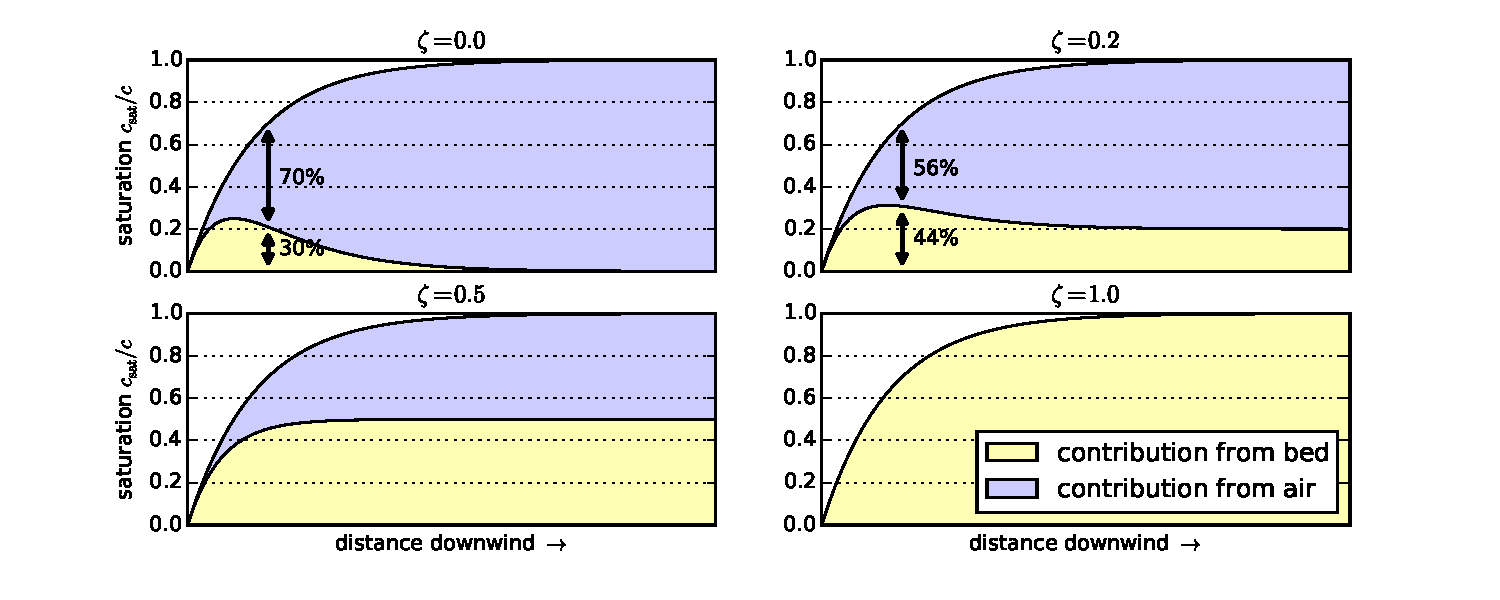
\includegraphics[width=\columnwidth]{../Figures/bed_interaction_parameter}
  \caption{Contributions of the grain size distribution in the bed and
    in the air to the weighting factors $\hat{w}_k$ for the
    equilibrium sediment concentration in Equation
    \ref{eq:erodep_multi} for different values of the bed interaction
    parameter.}
  \label{fig:bed_interaction_parameter}
\end{figure}

To allow for bed interaction in saturated situations in which no net
erosion can occur, the bed interaction parameter $\zeta$ is used (Figure
\ref{fig:bed_interaction_parameter}). The bed interaction parameter
can take values between 0.0 and 1.0 in which the weighting factors for
the equilibrium or saturated sediment concentration in an
(over)saturated situation are fully determined by the grain size
distribution in the bed or in the air respectively. A bed interaction
value of 0.2 represents the situation in which the grain size
distribution at the bed surface contributes 20\% to the weighting of
the saturated sediment concentration over the fractions. In the
example situation where the air is 70\% saturated such value for the
bed interaction parameter would lead to weighting factors that are
constituted for $70\% \cdot (100\% - 20\%) = 56\%$ based on the grain
size distribution in the air and for the other 44\% based on the grain
size distribution at the bed surface (Figure
\ref{fig:bed_interaction_parameter}, upper right panel).

The parameterization of the exchange of momentum between sediment
fractions is an aspect of saltation that is still poorly
understood. Therefore calibration of the bed interaction parameter
$\zeta$ is necessary. The model parameters in Equation
\ref{eq:equilibrium_transport} can be chosen in accordance with the
assumptions underlying multi-fraction sediment transport. $C$ should
be set to 1.5 as each individual sediment fraction is well-sorted,
$d_{\mathrm{n}}$ should be chosen equal to $D_{\mathrm{n}}$ as the
grain size dependency is implemented through
$u_{\mathrm{th}}$. $u_{\mathrm{th}}$ typically varies between 1 and 6
m/s for sand.

\subsection{Simulation of Sediment Sorting and Beach Armoring}

Since the equilibrium or saturated sediment concentration
$c_{\mathrm{sat},k}$ is weighted over multiple sediment fractions in
the extended advection model, also the instantaneous sediment
concentration $c_k$ is computed for each sediment fraction
individually. Consequently, grain size distributions may vary over the
model domain and in time. These variations are thereby not limited to
the horizontal, but may also vary over the vertical since fine
sediment may be deposited on top of coarse sediment or, reversely,
fines may be eroded from the bed surface leaving coarse sediment to
reside on top of the original mixed sediment. In order to allow the
model to simulate the processes of sediment sorting and beach armoring
the bed is discretized in horizontal grid cells and vertical bed
layers (2DV; Figure \ref{fig:bedcomposition}).

The discretization of the bed consists of a minimum of three vertical
bed layers with a constant thickness and an unlimited number of
horizontal grid cells. The top layer is the \textit{bed surface layer}
and is the only layer that interacts with the wind and hence
determines the spatiotemporal varying sediment availability and the
contribution of the grain size distribution in the bed to the weighting
of the saturated sediment concentration. One or more \textit{bed
  composition layers} are located underneath the bed surface layer and
form the upper part of the erodible bed. The bottom layer is the
\textit{base layer} and contains an infinite amount of erodible
sediment according to the initial grain size distribution. The base
layer cannot be eroded, but can supply sediment to the other layers.

\begin{figure}
  \centering
  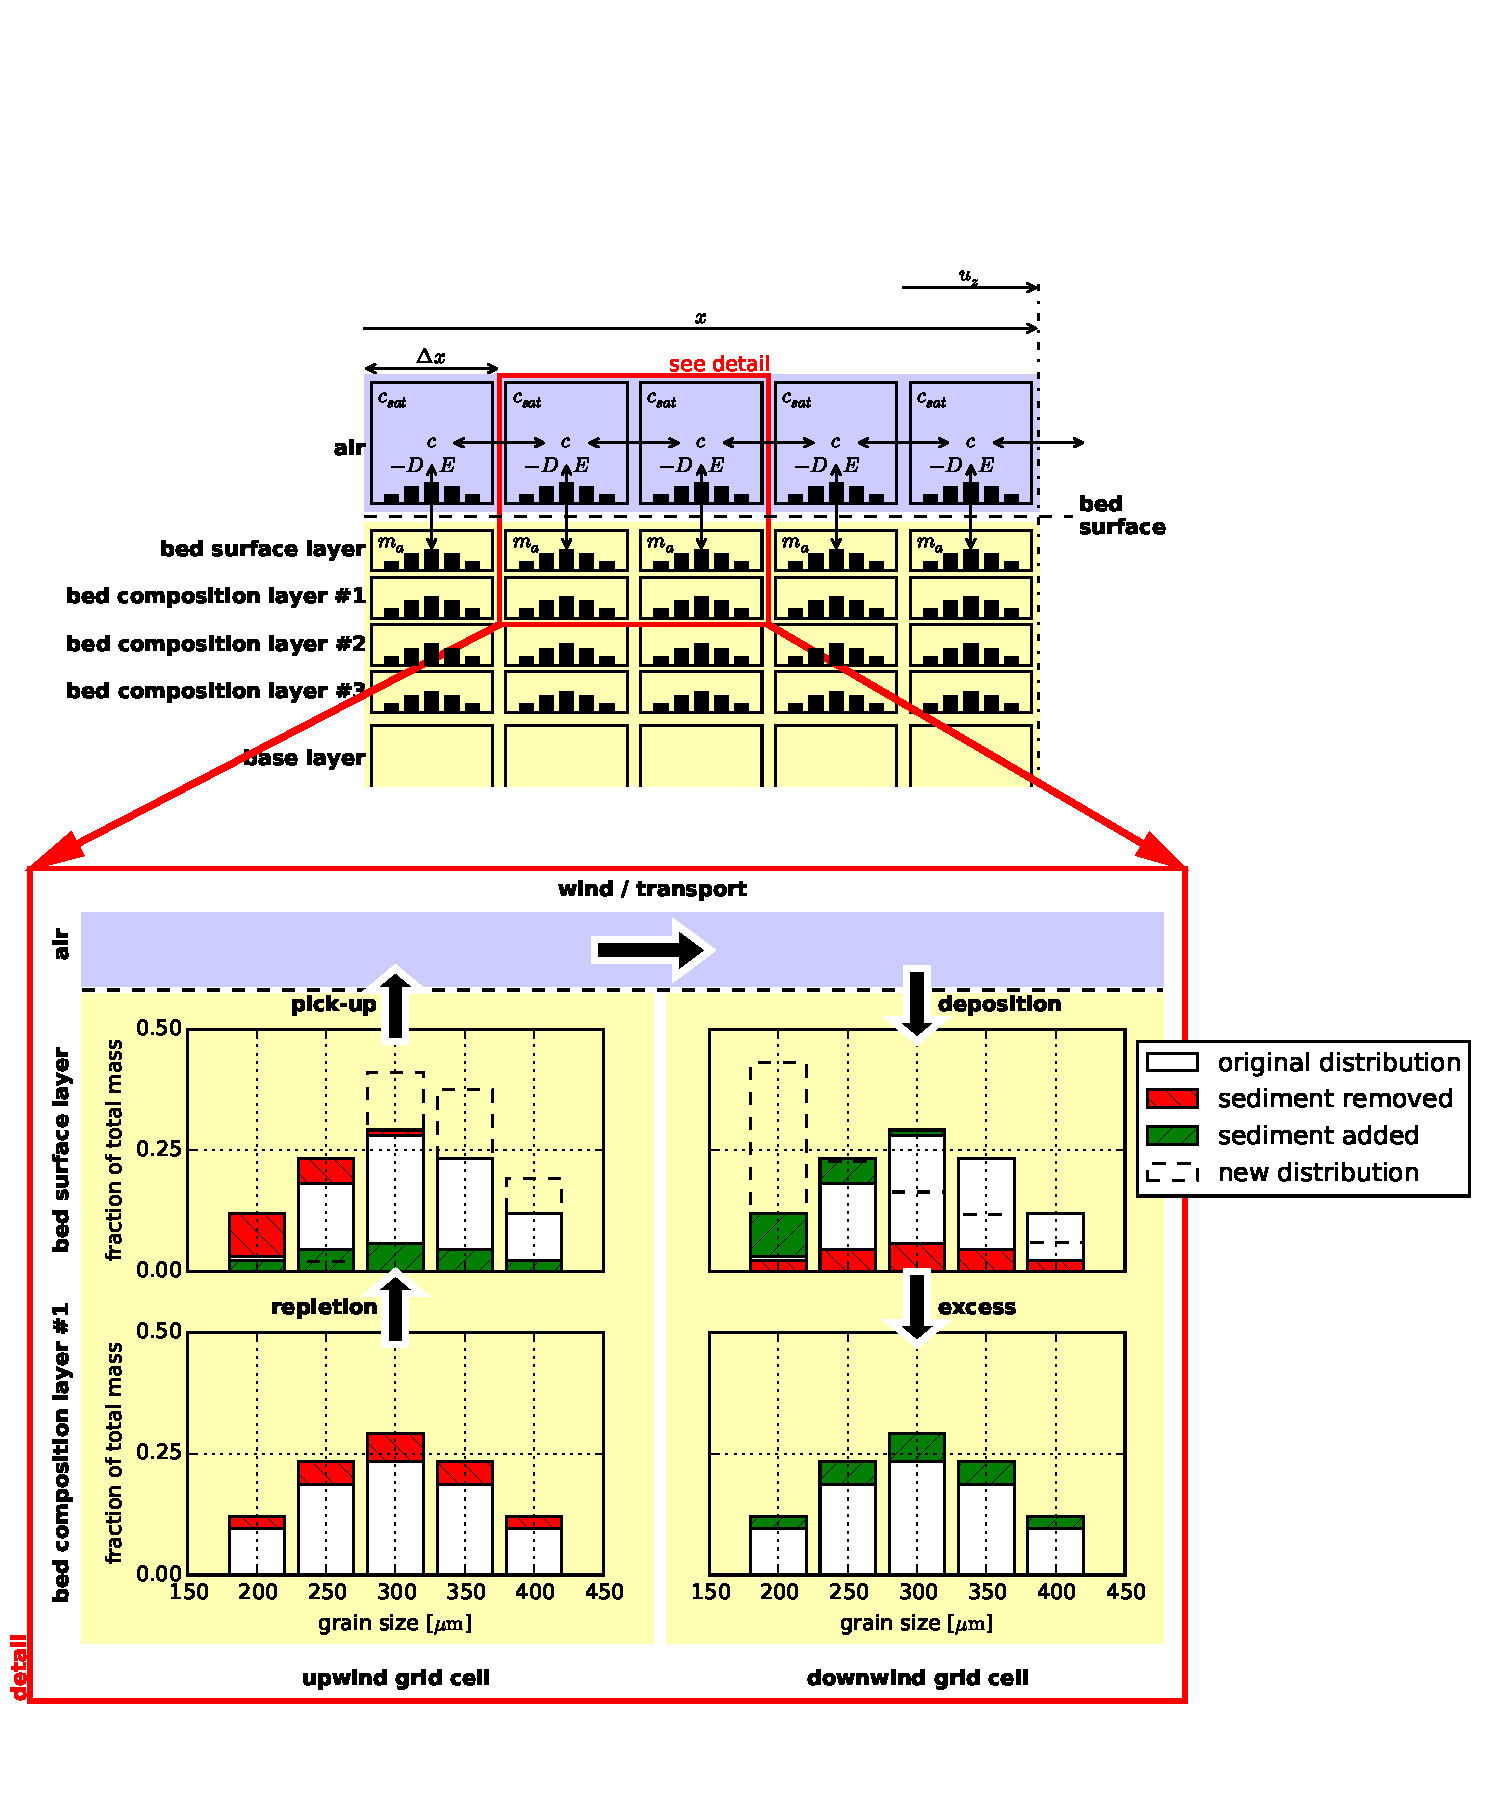
\includegraphics[width=\columnwidth]{../Figures/bedcomposition}
  \caption{Schematic of bed composition discretisation and advection
    scheme. Horizontal exchange of sediment may occur solely through
    the air that interacts with the \textit{bed surface layer}. The
    detail presents the simulation of sorting and beach armoring where
    the bed surface layer in the upwind grid cell becomes coarser due
    to non-uniform erosion over the sediment fractions, while the bed
    surface layer in the downwind grid cell becomes finer due to
    non-uniform deposition over the sediment fractions. Symbols refer
    to Equations \ref{eq:advection} and \ref{eq:erodep}.}
  \label{fig:bedcomposition}
\end{figure}

Each layer in each grid cell describes a grain size distribution over
a predefined number of sediment fractions (Figure
\ref{fig:bedcomposition}, detail). Sediment may enter or leave a grid
cell only through the bed surface layer. Since the velocity threshold
depends among others on the grain size, erosion from the bed surface
layer will not be uniform over all sediment fractions, but will tend
to erode fines more easily than coarse sediment (Figure
\ref{fig:bedcomposition}, detail, upper left panel). If sediment is
eroded from the bed surface layer, the layer is repleted by sediment
from the lower bed composition layers. The repleted sediment has a
different grain size distribution than the sediment eroded from the
bed surface layer. If more fines are removed from the bed surface
layer in a grid cell than repleted, the median grain size
increases. If erosion of fines continues the bed surface layer becomes
increasingly coarse. Deposition of fines or erosion of coarse material
may resume the erosion of fines from the bed.

In case of deposition the process is similar. Sediment is deposited in
the bed surface layer that then passes its excess sediment to the
lower bed layers (Figure \ref{fig:bedcomposition}, detail, upper right
panel). If more fines are deposited than passed to the lower bed
layers the bed surface layer becomes increasingly fine.

\subsection{Simulation of the Emergence of Non-erodible Roughness
  Elements} \label{sec:roughness}

Sediment sorting may lead to the emergence of non-erodible elements
from the bed. Non-erodible roughness elements may shelter the
erodible bed from wind erosion due to shear partitioning, resulting in
a reduced sediment availability \citep{Raupach1993}. Therefore
Equation \ref{eq:raupach} is implemented according to:

\begin{equation} \label{eq:raupach2}
u_{\mathrm{* th, R}} = u_{\mathrm{* th}} \cdot \sqrt{ \left( 1 - m \cdot \sum_{k=k_0}^{n_{\mathrm{k}}}{w_k^{\mathrm{bed}}} \right) \left( 1 + \frac{m \beta}{\sigma} \cdot \sum_{k=k_0}^{n_{\mathrm{k}}}{w_k^{\mathrm{bed}}} \right) }
\end{equation}

\noindent in which $\sigma$ is the ratio between the frontal area and
the basal area of the roughness elements and $\beta$ is the ratio
between the drag coefficients of the roughness elements and the bed
without roughness elements. $m$ is a factor to account for the
difference between the mean and maximum shear stress and is usually
chosen 1.0 in wind tunnel experiments and may be lowered to 0.5 for
field applications. The roughness density $\lambda$ in the original
equation of \citet[][Equation \ref{eq:raupach}]{Raupach1993} is
obtained from the mass fraction in the bed surface layer $w_k^{\mathrm{bed}}$
(Equation \ref{eq:massfraction}) according to:

\begin{equation}
\label{eq:roughness_density}
\lambda = \frac{\sum_{k=k_0}^{n_{\mathrm{k}}}{w_k^{\mathrm{bed}}}}{\sigma}
\end{equation}

\noindent in which $k_0$ is the index of the smallest non-erodible
sediment fraction in current conditions and $n_{\mathrm{k}}$ is the
total number of sediment fractions. It is assumed that the sediment
fractions are ordered by increasing size. Whether a fraction is
erodible depends on the sediment transport capacity.

\subsection{Simulation of the Hydraulic Mixing, Infiltration and
  Evaporation} \label{sec:marine_processes}

As sediment sorting due to aeolian processes can lead to armoring of a
beach surface, mixing of the beach surface or erosion of course
material may undo the effects of armoring. To ensure a proper balance
between processes that limit and enhance sediment availability in the
model both types of processes need to be sufficiently represented when
simulating spatiotemporal varying bed surface properties and sediment
availability.

A typical upwind boundary in coastal environments during onshore winds
is the water line. For aeolian sediment transport the water line is a
zero-transport boundary. In the presence of tides, the intertidal
beach is flooded periodically. Hydraulic processes like wave breaking
mix the bed surface layer of the intertidal beach, break the beach
armoring and thereby influence the availability of sediment. Moreover,
the hydraulic processes periodically wet the intertidal beach
temporally increasing the shear velocity threshold. Infiltration and
evaporation subsequently dry the beach.

In the model the mixing of sediment is simulated by averaging the
sediment distribution over the depth of disturbance
($\Delta z_{\mathrm{d}}$). The depth of disturbance is linearly
related to the breaker height \citep[e.g.][]{King1951, Williams1971,
  Masselink2007}. \citet{Masselink2007} proposes an empirical factor
$f_{\Delta z_{\mathrm{d}}}$ [-] that relates the depth of disturbance
directly to the local breaker height according to:

\begin{equation}
  \label{eq:dod}
  \Delta z_{\mathrm{d}} = f_{\Delta z_{\mathrm{d}}} \cdot \min \left ( H \quad ; \quad \gamma \cdot d \right )
\end{equation}

\noindent in which the offshore wave height $H$ [m] is taken as the
local wave height maximized by a maximum wave height over depth ratio
$\gamma$ [-]. $d$ [m] is the water depth that is provided to the model
through an input time series of water levels. Typical values for
$f_{\Delta z_{\mathrm{d}}}$ are 0.05 to 0.4 and 0.5 for $\gamma$.

The drying of the beach is simulated by simplified functions for
infiltration and evaporation. Infiltration is represented by an
exponential decay function that is governed by a drying time scale
$T_{\mathrm{dry}}$. Evaporation is simulated using an adapted version
of the Penman-Monteith equation \citep{Shuttleworth1993} that is
governed by meteorological time series of solar radiation, temperature
and humidity.

\section{Results} \label{sec:results}

The model is applied to a series of prototype cases to illustrate the
processes described by the model, two wind tunnel experiments to
illustrate the capabilities of the model to simulate spatiotemporal
variations in bed surface properties and sediment availability and a
sensitivity analysis.

\subsection{Prototype cases} \label{sec:prototype}

The four prototype cases P1 to P4 are intended to illustrate the
capabilities of the presented model to simulate processes of sediment
sorting \citep{VanDerWal2000, Arens2002} and beach armoring
\citep{VanDerWal1998}. The prototype cases are constructed using a 120
m schematized linear beach with a 1:20 slope, a wind velocity of 12 or
30 m/s, a drying time scale $T_{\mathrm{dry}}$ of 3 h, constant
evaporation and a simulation time of 30 days. The prototype cases are
initialized with lognormally distributed sediment with $d_{50} = 335$
$\mu \mathrm{m}$ ($\Phi-\mathrm{scale} = 1.6$, $\sigma_{\Phi} = 0.4$),
which is representative for nourished poorly sorted beaches along the
Dutch coast.  Parameterizations for shells and shell fragments in
Equation \ref{eq:raupach2} are based on experiments described by
\citet{McKennaNeuman2012} and chosen as $m = 0.5$, $\sigma = 4.2$ and
$\beta = 130$. The four scenarios described by the prototype cases
are:

\begin{description}
\item[P1] This scenario is used as reference for normalization and
  involves sand only and no tidal movement. The model is forced by a
  constant wind of 12 m/s. Sediment sorting occurs due to the presence
  of a wide range of sediment fractions. However, beach armoring does
  not occur due to the absence of shells, resulting in an almost
  constant sediment transport rate at the downwind end of the domain.
\item[P2] This scenario involves 5\% of shells and shell fragments
  ranging from 2 to 30 mm and no tidal movement. The model is forced
  by a constant wind of 12 m/s. The presence of shells means that beach
  armoring occurs that causes spatiotemporal variations in sediment
  availability and a decrease in sediment transport.
\item[P3] This scenario involves 5\% of shells and shell fragments and
  a sinusoidal tide with a 2 m tidal range and a tidal period of 12
  h. The tide periodically floods a 40 m intertidal beach area. The
  model is forced by a constant wind of 12 m/s. The tidal movement
  causes mixing of the bed surface layer in the intertidal beach area
  reducing the effects of beach armoring.
\item[P4] This scenario is equal to scenario P3, but the model is
  forced by a wind of 12 m/s that is increased twice to 30 m/s to
  simulate the effect of higher energy wind events that (partially)
  reset the composition of the bed surface layer and temporarily
  increase the sediment availability in the dry beach area.
\end{description}

\begin{figure}
  \centering
  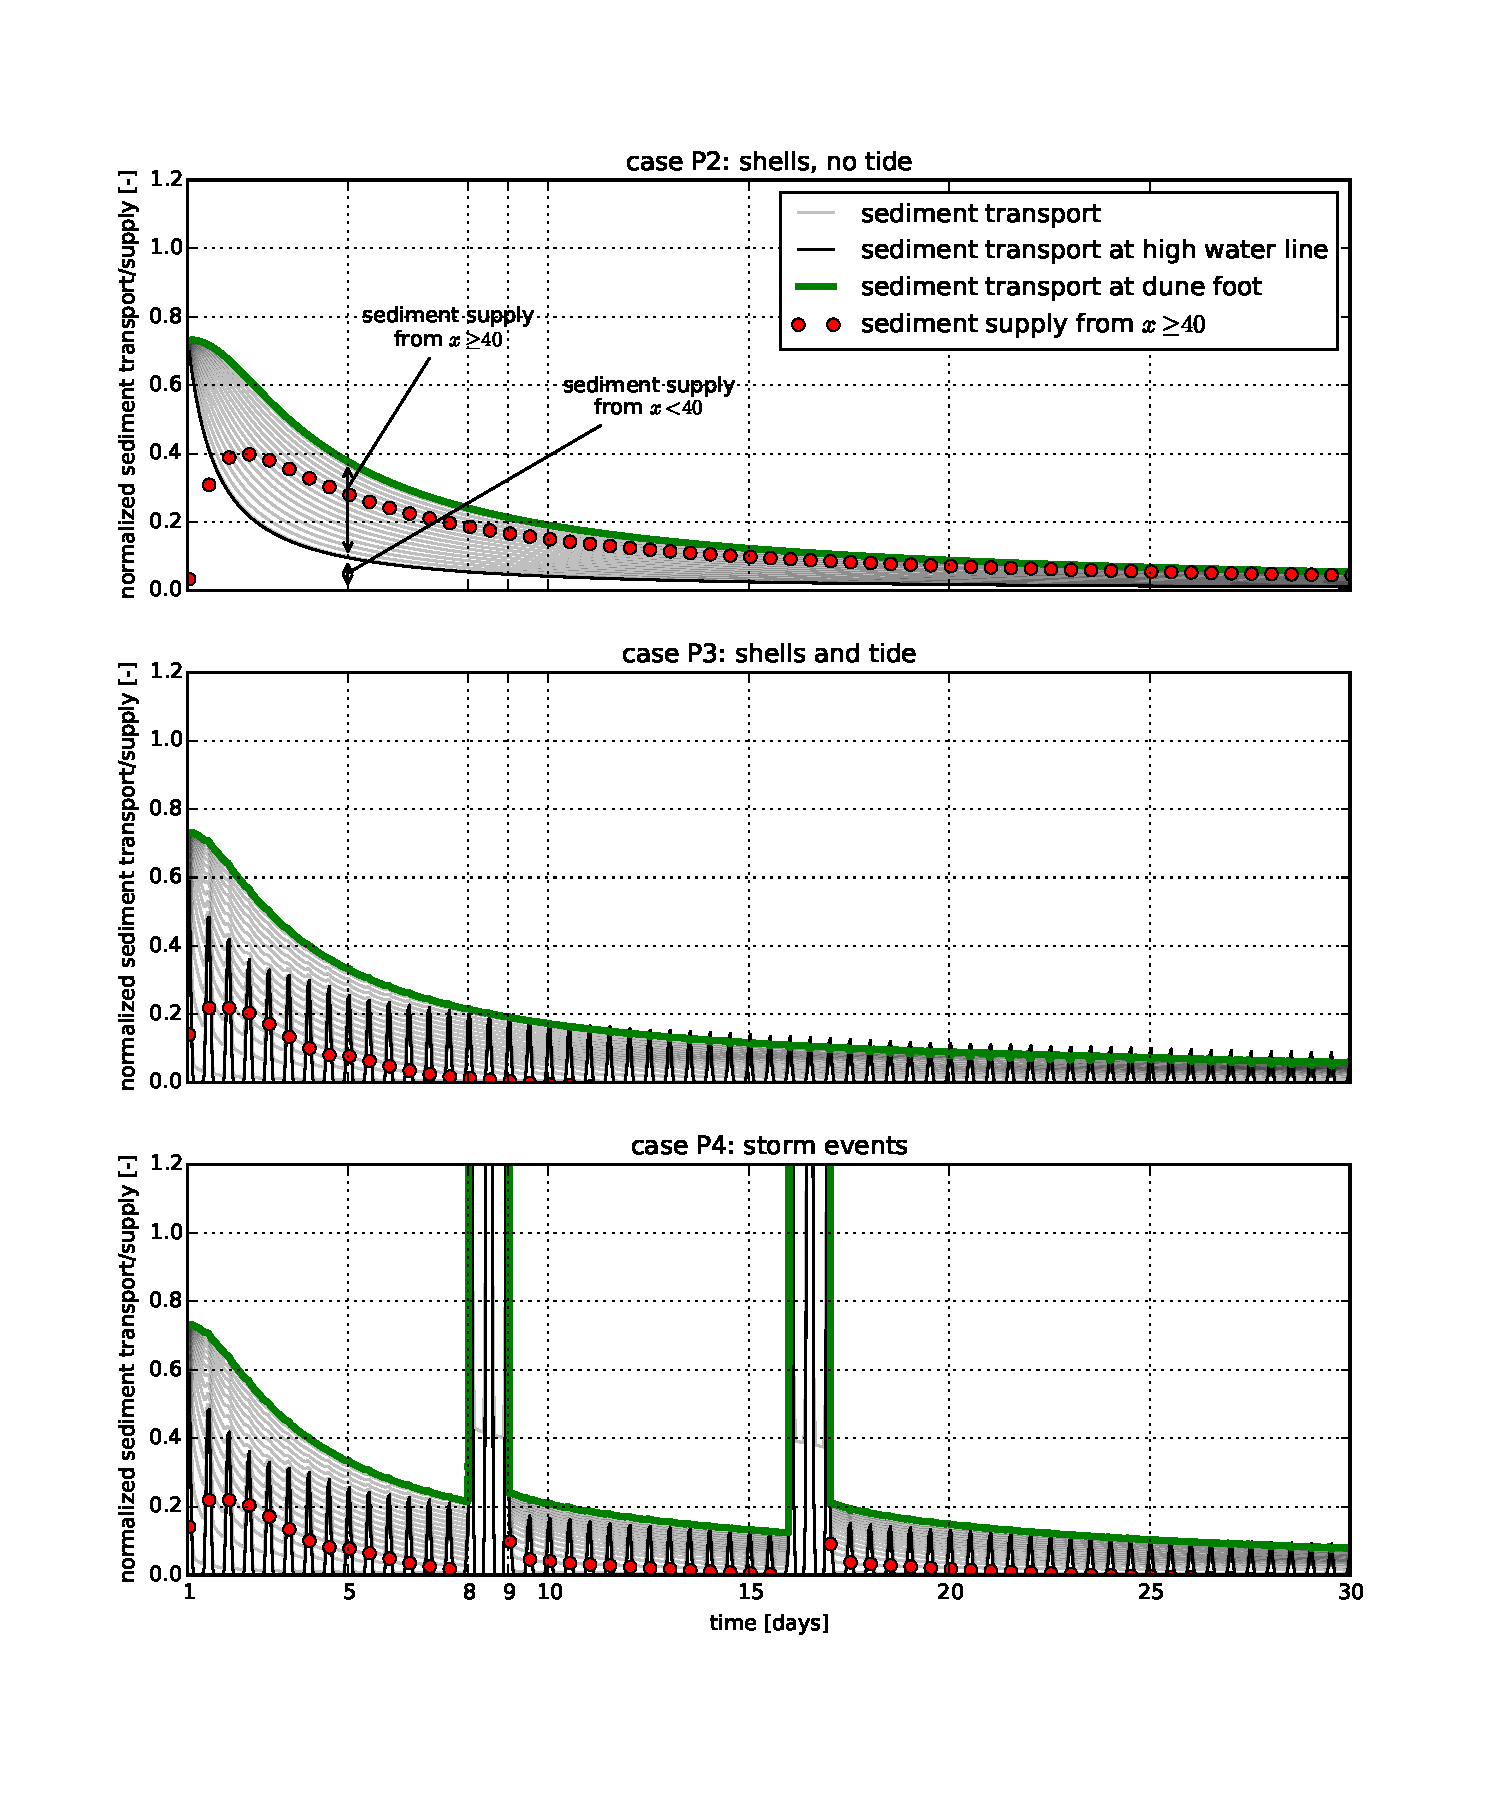
\includegraphics[width=\columnwidth]{../Figures/transport_rate_v2}
  \caption{Sediment transport in time and over the model domain for
    three scenarios with constant wind. Each line depicts a different
    location along the beach, starting from $x = 40$ m, which
    coincides with the high water line in cases P3 and P4, and ends at
    the dune foot. Results are normalized using the transport rate in
    case P1 with almost constant transport (not shown). The difference
    between the sediment transport at dune foot (green) and the
    sediment transport at $x = 40$ m is visualized by the red dots and
    represents the sediment supply from the dry beach. In cases P3 and
    P4 the sediment transport at the high water line periodically
    exceeds the sediment transport at the dune foot, indicating local
    deposition of sediments originating from the intertidal beach.}
  \label{fig:transport_rate}
\end{figure}

\begin{figure}
  \centering
  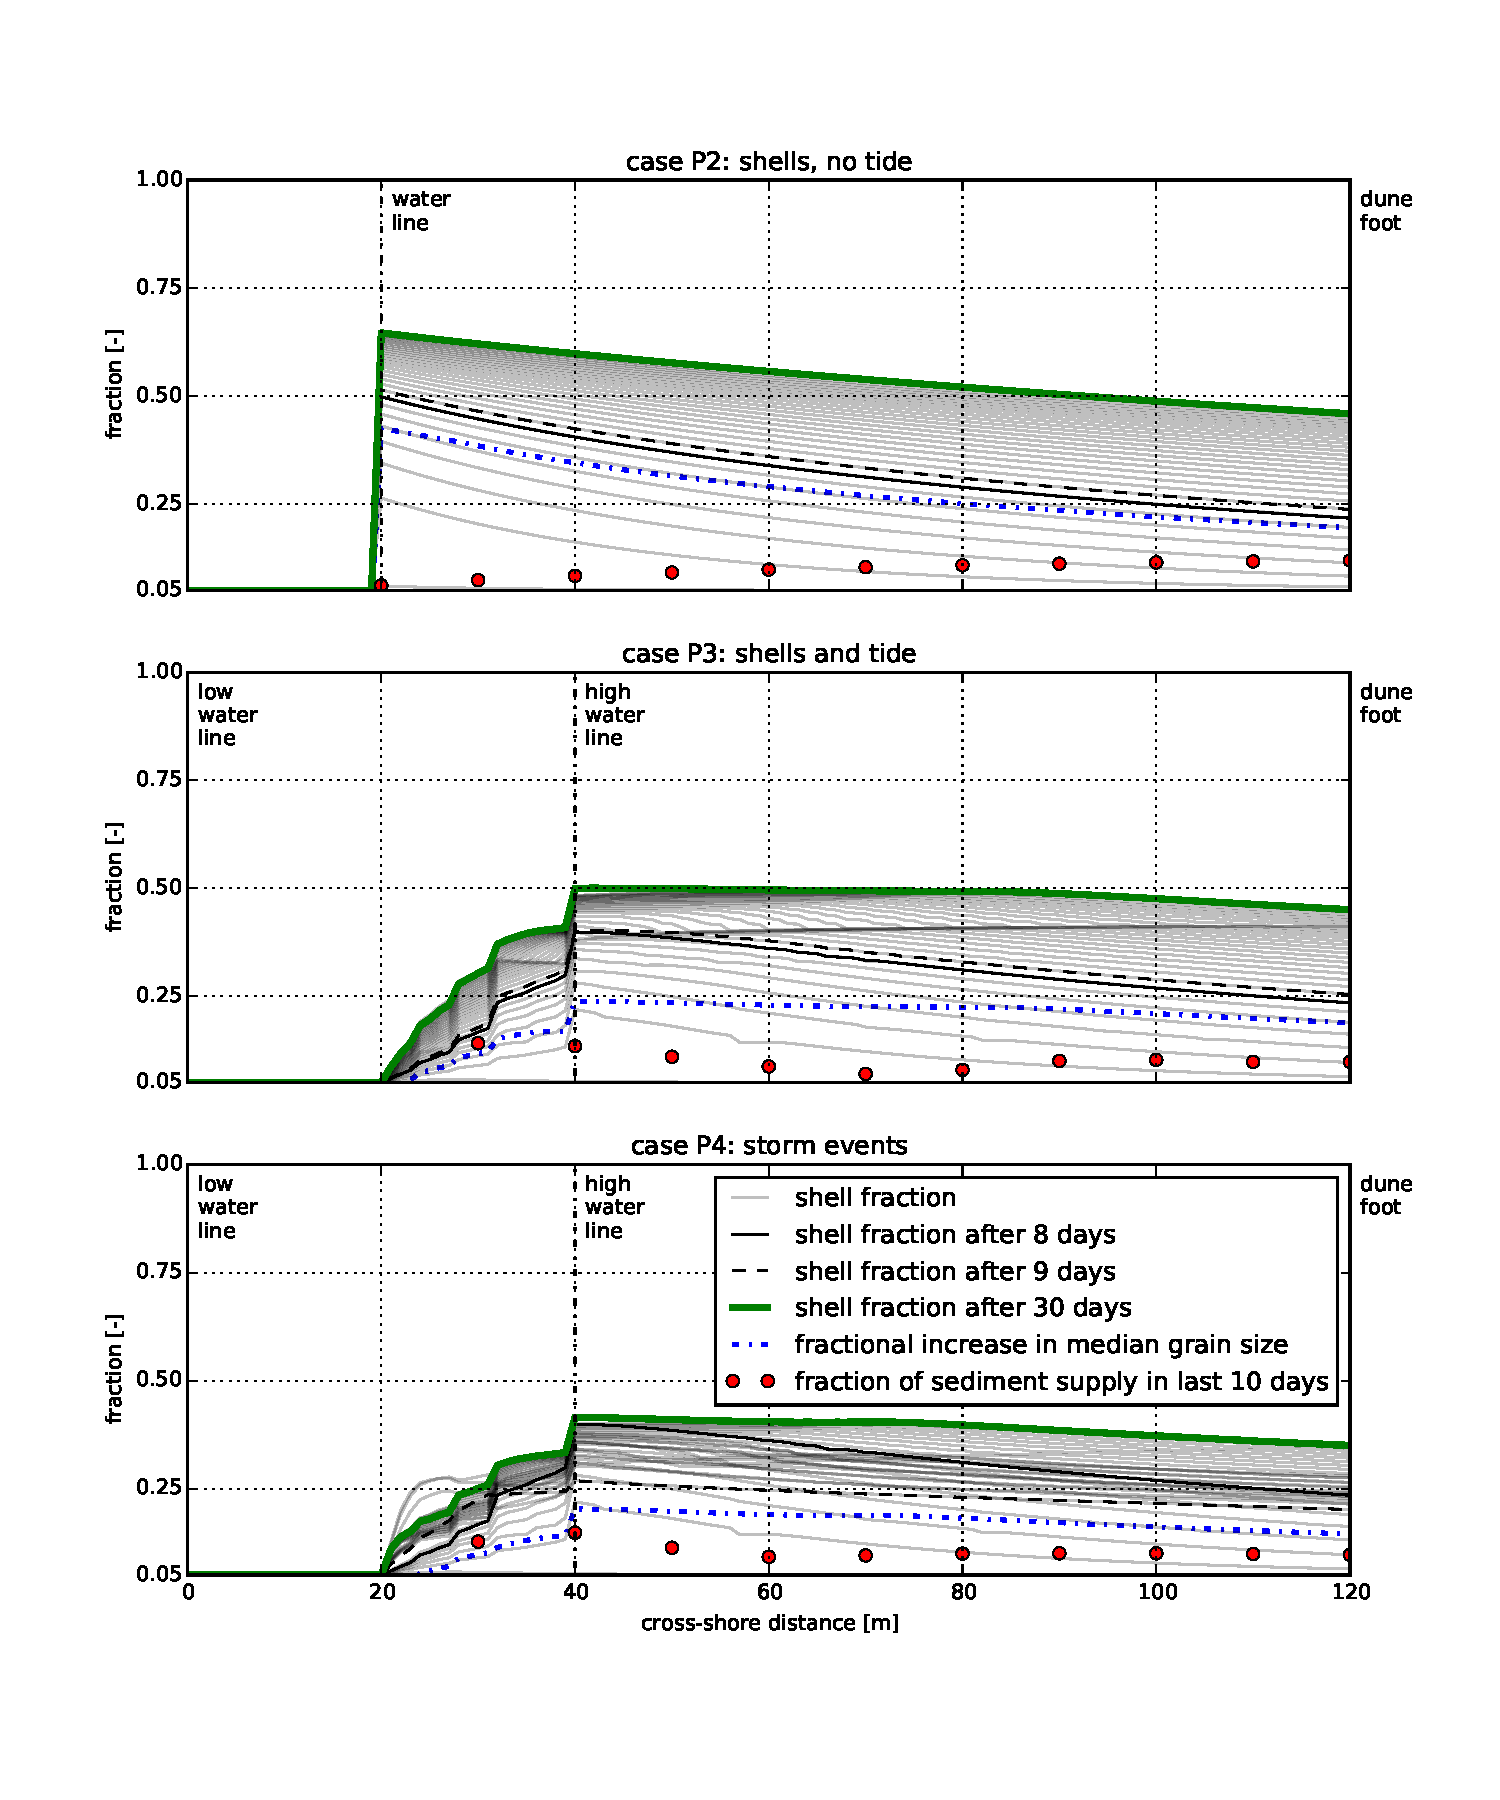
\includegraphics[width=\columnwidth]{../Figures/shell_fraction}
  \caption{Distribution of the shell fraction over the model domain
    and in time. Sediment supply is inversely related to the degree of
    beach armoring, indicated by the shell fraction. Median grain size
    increases with the increase in shell fraction indicating erosion
    of predominantly fines. High-energy wind events in case P4 even
    mobilize shell fractions resulting in a decrease in beach armoring
    and an increase in sediment availability.}
  \label{fig:shell_fraction}
\end{figure}

Figure \ref{fig:transport_rate} presents the simulated aeolian
sediment transport rates at the downwind end of the domain for cases
P2 to P4 over the course of 30 days of simulation time. The results
are normalized using the transport rate in case P1. The reference case
P1 shows an almost constant transport rate over the entire course of
the simulation. The presence of shells in case P2 results in a
reduction of sediment availability. As a result, the transport rates
in case P2 are lower compared to case P1. The transport rate decreases
as more shells emerge from the bed and a beach armor layer
develops. In case P2 there are no processes that break the armoring
and the transport rates asymptotically reach zero. The beach armor
layer develops in direction of the wind. Therefore, the relative
contribution of the downwind part of the beach ($x \geq 40$) to the
total sediment transport increases over time.

Case P3 includes tidal movement and hydraulic mixing. At the high
water line the sediment transport is zero during high tide and
maximized during low tide. Initially, transport is not saturated at
the high water line and entrainment of sediment continues over the dry
beach. As shells emerge from the bed, a beach armor layer develops
that reduces sediment availability. The reduction of sediment
availability progresses slower at the intertidal beach compared to the
dry beach due to hydraulic mixing. After 8 days the sediment transport
rates at the high water line start to exceed the sediment transport
rates at the dune foot during low water. Sediment that is eroded from
the intertidal beach during low water is partially trapped at the dry
beach due to differences in roughness. During subsequent high water,
when the sediment supply from the intertidal beach ceases, these
deposits are again entrained and blown downwind. The net erosion from
the dry beach ultimately approaches zero as armoring of the dry beach
progresses. At this point all sediment deposited downwind originates
directly from the intertidal beach. However, due to the spatial
differences in roughness, sediment is temporally deposited at the dry
beach and cause the sediment transport rates at the dune foot to be
only weakly correlated with the tidal movement.

Case P4 shows a pattern similar to case P3, but after 8 and 16 days a
relatively high-energy wind event passes for 24 hours. As a result,
the transport rate spikes, but an elevated transport rate is also
visible after the wind velocity drops.  During the high-energy wind
event even small shell fragments are mobilized. The beach armoring is
therefore (partially) removed and more sediment is available for
transportation afterwards. This leads to a prolonged peak in sediment
transport and an increase of the relative contribution of the dry
beach to the total sediment transport at the dune foot. After the
beach armoring is re-established over time the transport rates
approach the rates of case P3 again.

The differences in transport rate between the prototype cases are
directly related to sediment availability, since the wind is constant
in all cases but case P4. Figure \ref{fig:shell_fraction} shows the
fractions of shells and shell fragments in the bed surface layer for
case P2 to P4. The shell fraction increases over time in all
simulations. In case P2 the shell fraction peaks at the water line as
the beach armor layer develops in downwind direction. Consequently, at
the end of the simulation most sediment originates from the downwind
end of the beach where the beach armoring is least developed. In case
P3 and P4 hydraulic mixing causes the shell fraction in the intertidal
beach to remain low resulting in a different distribution of shells
compared to case P2 and hence a difference in sediment
availability. Consequently, at the end of the simulation most sediment
originates from the intertidal beach. In reality, the contribution of
the intertidal beach to the total sediment transport is likely to be
higher as more marine processes counteract the local development of a
beach armor layer than currently simulated, like marine deposits and
buoyancy of shells. In case P4 the drop in shell fraction from day 8
to day 9 is related to the first high-energy wind event. At the end of
the simulation, the fraction of sediment that originates from the
intertidal beach is relatively low compared to case P3. In all cases
also the median grain size in the bed surface layer increases,
indicating that predominantly fine sediment is eroded from the
bed. The unbalanced sediment transport over the fractions cause
sediment sorting in downwind direction.

%The prototype cases illustrate the potential importance of beach
%armoring for aeolian sediment transport estimates and the location of
%sediment source areas. Multi-fraction sediment transport drives the
%spatiotemporal variations in sediment availability due to the
%development of a beach armor layer. In addition, multi-fraction
%sediment transport simulates sorting of sediment in downwind
%direction.

The contribution to the instantaneous sediment transport of the
specific processes described by the model can be distinguished in the
prototype cases P1 to P4 because a constant wind velocity is
imposed. If a more realistic variable wind velocity time series is
used, the contributions of the specific processes are obscured by the
wind-related variance. To show that the simulation of spatiotemporal
bed surface properties and sediment are also important in variable
wind conditions, prototype cases P1 to P3 are repeated using an
synthetic variable wind time series (P1b to P3b). The time series is
generated using a Markov Chain Monte Carlo (MCMC) simulation following
a Weibull distribution with a mean wind velocity of 12 m/s.

Figure \ref{fig:variable_wind} shows the sediment transport rate in
case P3b normalized by the sediment transport rate in case P1b
depending on the hourly averaged wind velocity. To remove the
influence of the wind variability, the normalized sediment transport
time series obtained from the simulations are binned according to the
hourly averaged wind velocity in 0.5 m/s bins. The median transport
rate in each bin is subsequently determined to obtain a relation
between instantaneous normalized sediment transport and wind
velocity. The reduction is close to 100\% up to wind velocities of 5
m/s and subsequently decreases according to an exponential
function. The median reduction for 12 m/s wind velocity is 74\%, which
is less than the maximum reduction of 95.0\% with a constant 12 m/s
wind velocity in case P3. The reduction tends to increase during the
simulation as beach armoring progresses.

\begin{figure}
  \centering
  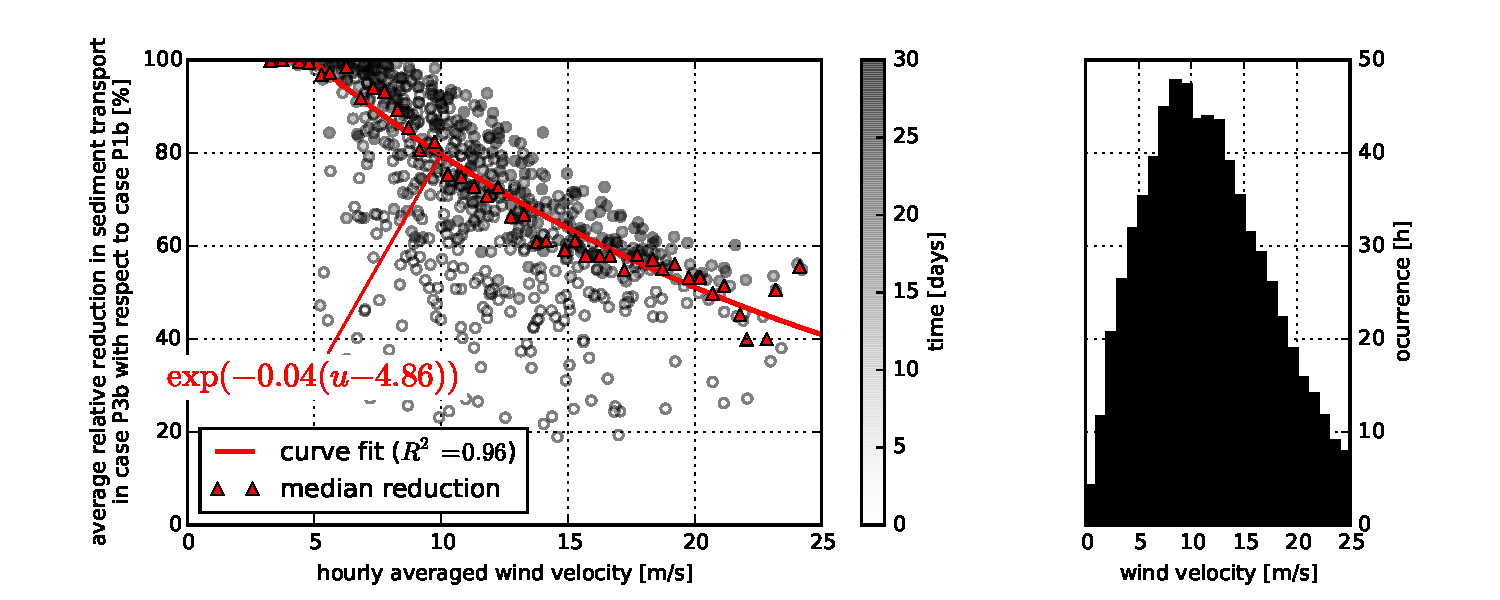
\includegraphics[width=\columnwidth]{../Figures/variable_wind_py}
  \caption{Average reduction in sediment transport in prototype case
    P3b compared to case P1b depending on the hourly averaged wind
    velocity (left panel). The results are obtained using an synthetic
    variable wind time series following a Weibull distribution with a
    mean wind velocity of 12 m/s (right panel). The sediment transport
    reduction (scatter) is binned according to the wind velocity using
    0.5 m/s bins. The median reduction per bin (triangles) is used to
    fit an exponential curve (line). The reduction tends to increase
    during the simulation (scatter colors).}
  \label{fig:variable_wind}
\end{figure}

\subsection{Wind tunnel experiments} \label{sec:windtunnel}

To illustrate the applicability of the model approach, two unrelated
wind tunnel experiments obtained from literature are simulated that
involve either temporal \citep{Nickling1995} or spatial
\citep{Dong2004b} variations in bed surface properties as discussed in
section \ref{sec:challenges}.

\citet{Nickling1995} describe an experiment in a wind tunnel with a
4.5 m working section in which a grid of 18 mm marbles was buried in
sandy material with $d_{50} = 270$ $\mu \mathrm{m}$.  During the
experiment with constant wind of 8 m/s, measured at 25 cm above the
bed, the sand is winnowed from in between the marbles resulting in the
emergence of the marbles over time. The emergence of the marbles cause
the bed to become armored. The effect of armoring of a marble extends
beyond the marble dimensions due to shadowing effects in the lee of
the marble described by Equation \ref{eq:raupach2}. All parameter
values, including $z'$, are obtained from \citet{Nickling1995} and
hence no further calibration of parameters is performed for this
simulation.

Figure \ref{fig:nickling1995} shows the modeled normalized sediment
transport rate in comparison with the measurements described in
\citet{Nickling1995}. Where the measurements start with a relatively
constant transport and even a slight increase in transport, the model
predicts an immediate decrease in transport. The marbles are modeled
as a large sediment fraction for which its presence in a bed
composition layer is described by a mass fraction rather than a
location. Therefore, it is possible to define the marble density, but
not the exact marble locations. Consequently, from the start of the
simulation marbles start to emerge from the bed resulting in an
immediate decrease in sediment transport. In contrast, in the wind
tunnel the marbles are covered with a thin layer of sand that was
removed first before the marbles start to emerge. The initial
emergence of the marbles coincided with a slight increase in sediment
transport. \citet{Nickling1995} attributes this rise to a pronounced
change in boundary conditions and turbulence. Since these small scale
variations in the wind shear are not represented in the model the rise
in transport is not visible in the model results. However, the
decrease in sediment transport due to the emergence of the marbles for
the three different grid spacings described in \citet{Nickling1995},
is qualitatively represented by the model.

\citet{Dong2004b} describe an experiment in a wind tunnel with a 21 m
working section in which a patch of gravel with diameter 10 -- 40 mm
was positioned downwind of a sandy bed with $d_{50} = 180$
$\mu \mathrm{m}$. The length of the gravel patch was varied between
the experiments from 0.5 -- 12 m and the wind velocity from 8 -- 22
m/s, measured at 60 cm above the bed. The free-flow wind velocities
are converted to shear velocities assuming $z'$ = 6 mm. The gravel
patch traps saltating grains. In the model the entrapment of grains is
simulated as an exchange of momentum between the sandy fractions and
the immobile gravel fraction. This exchange is governed by the bed
interaction parameter, which is calibrated for this simulation and
found to be 0.05.

Figure \ref{fig:dong2004} shows the modeled sediment transport rate in
comparison with the measurements described in \citet{Dong2004b}. The
increase in sediment transport with increasing wind velocity is well
represented by the model given the uniform RMSE among the different
wind velocities. The decrease in sediment transport rate with
increasing gravel patch length is represented by the model with a
relative RMSE of less than 10\% for all except the lowest and highest
wind velocities. Significant surpassing of sediment over the sediment
trap during the measurements with 22 m/s wind velocity is reported by
\citet{Dong2004b}, which explains the consistent overprediction of the
sediment fluxes by the model. The discrepancy between the model and
the measurements for the 8 and 10 m/s wind velocities is less
consistent and is expected to be a result of a low signal-to-noise
ratio related to the small sediment fluxes. Also for short gravel
patch lengths the model deviates from the measurements. The relatively
high variability over the 0.5 to 2 m gravel patch lengths is
attributed to a change in transport characteristics \citep{Dong2004b}
due to fully elastic collisions between the sand grains and the
gravel. A bed interaction parameter that is not constant is needed to
capture this behavior in the model.

\begin{figure}
  \centering
  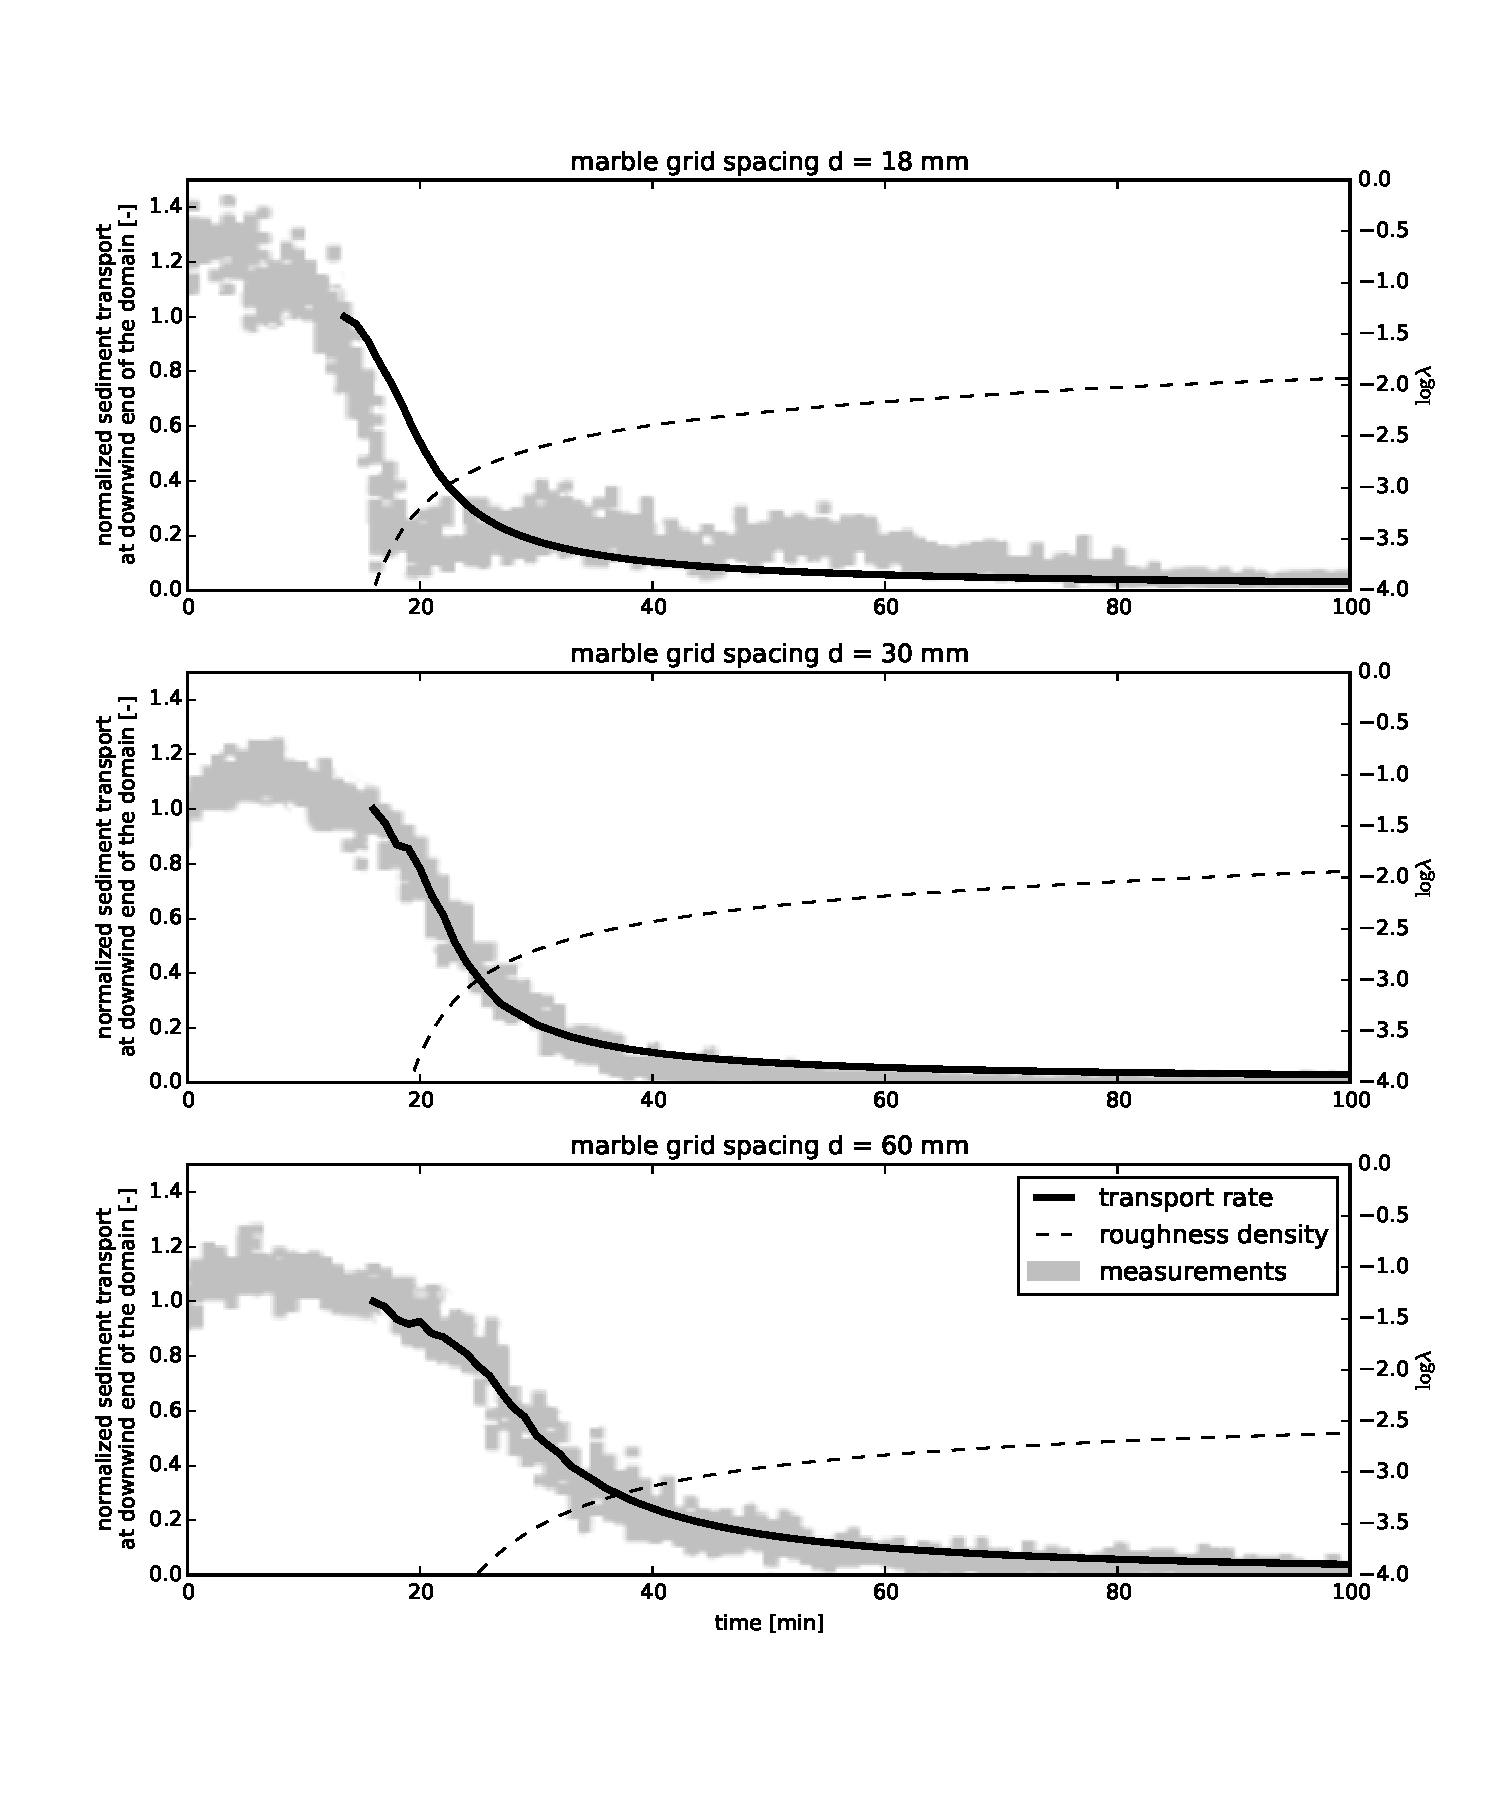
\includegraphics[width=\columnwidth]{../Figures/nickling1995_py}
  \caption{Comparison between modeled and measured normalized sediment
    transport rates from wind tunnel experiments described in
    \citet{Nickling1995}. The dashed line depicts the emergence of
    marbles in terms of increasing roughness density. The
    visualization of the measurement results is copied from Figure 4
    in the original publication without digitization.}
  \label{fig:nickling1995}
\end{figure}

\begin{figure}
  \centering
  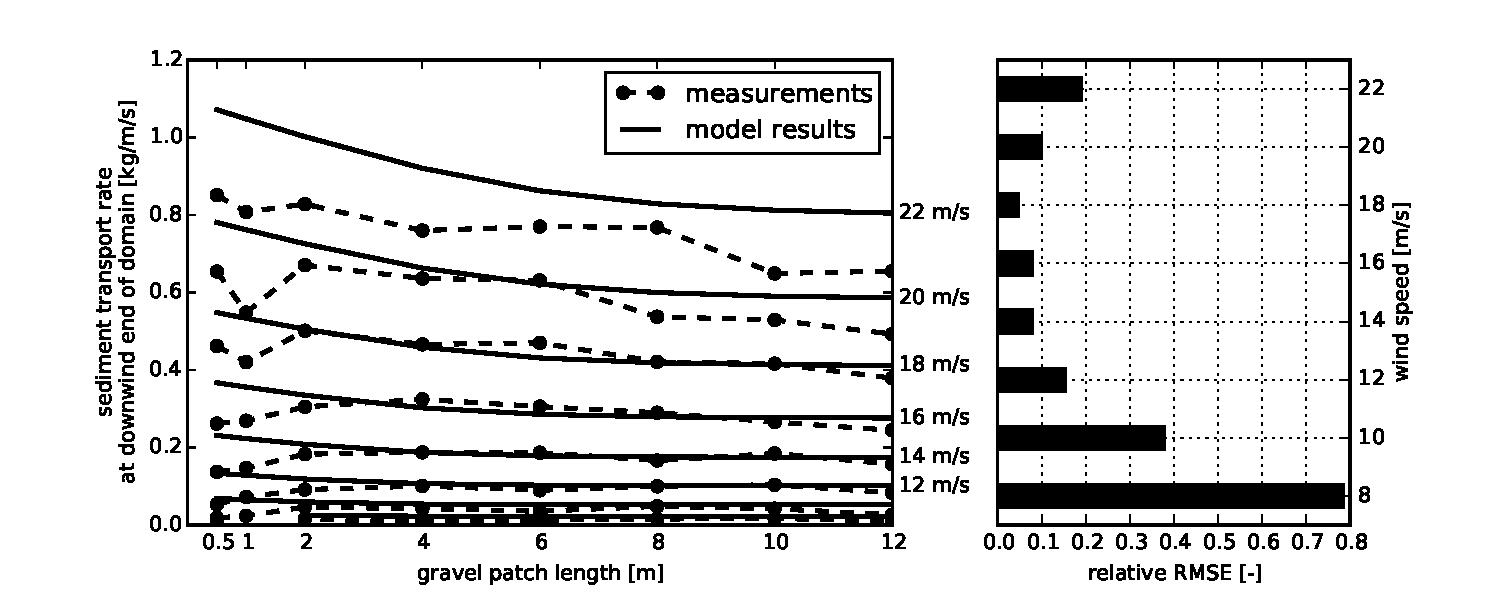
\includegraphics[width=\columnwidth]{../Figures/dong2004_py}
  \caption{Comparison between model results and measurements from wind
    tunnel experiments described in \citet{Dong2004b} (left panel) and
    RMS errors relative to the mean measured transport rate (right
    panel). The measured transport rates with a wind velocity of 22
    m/s are underestimated due to surpassing of sediment over the
    sediment trap \citep{Dong2004b}.}
  \label{fig:dong2004}
\end{figure}

\subsection{Sensitivity}

The sensitivity of the model to four newly introduced parameters and
the wind velocity is determined to obtain insight in the importance of
these parameters to the model results. The newly introduced parameters
are the bed interaction parameter, depth of disturbance factor, the
drying time scale and the grain size distribution standard
deviation. Case P3 as presented in section \ref{sec:prototype} is used
as starting point for the sensitivity analysis. Figure
\ref{fig:sensitivity} shows the change in normalized total sediment
transport given variations of each of the four model parameters and
the wind velocity.

\begin{figure}
  \centering
  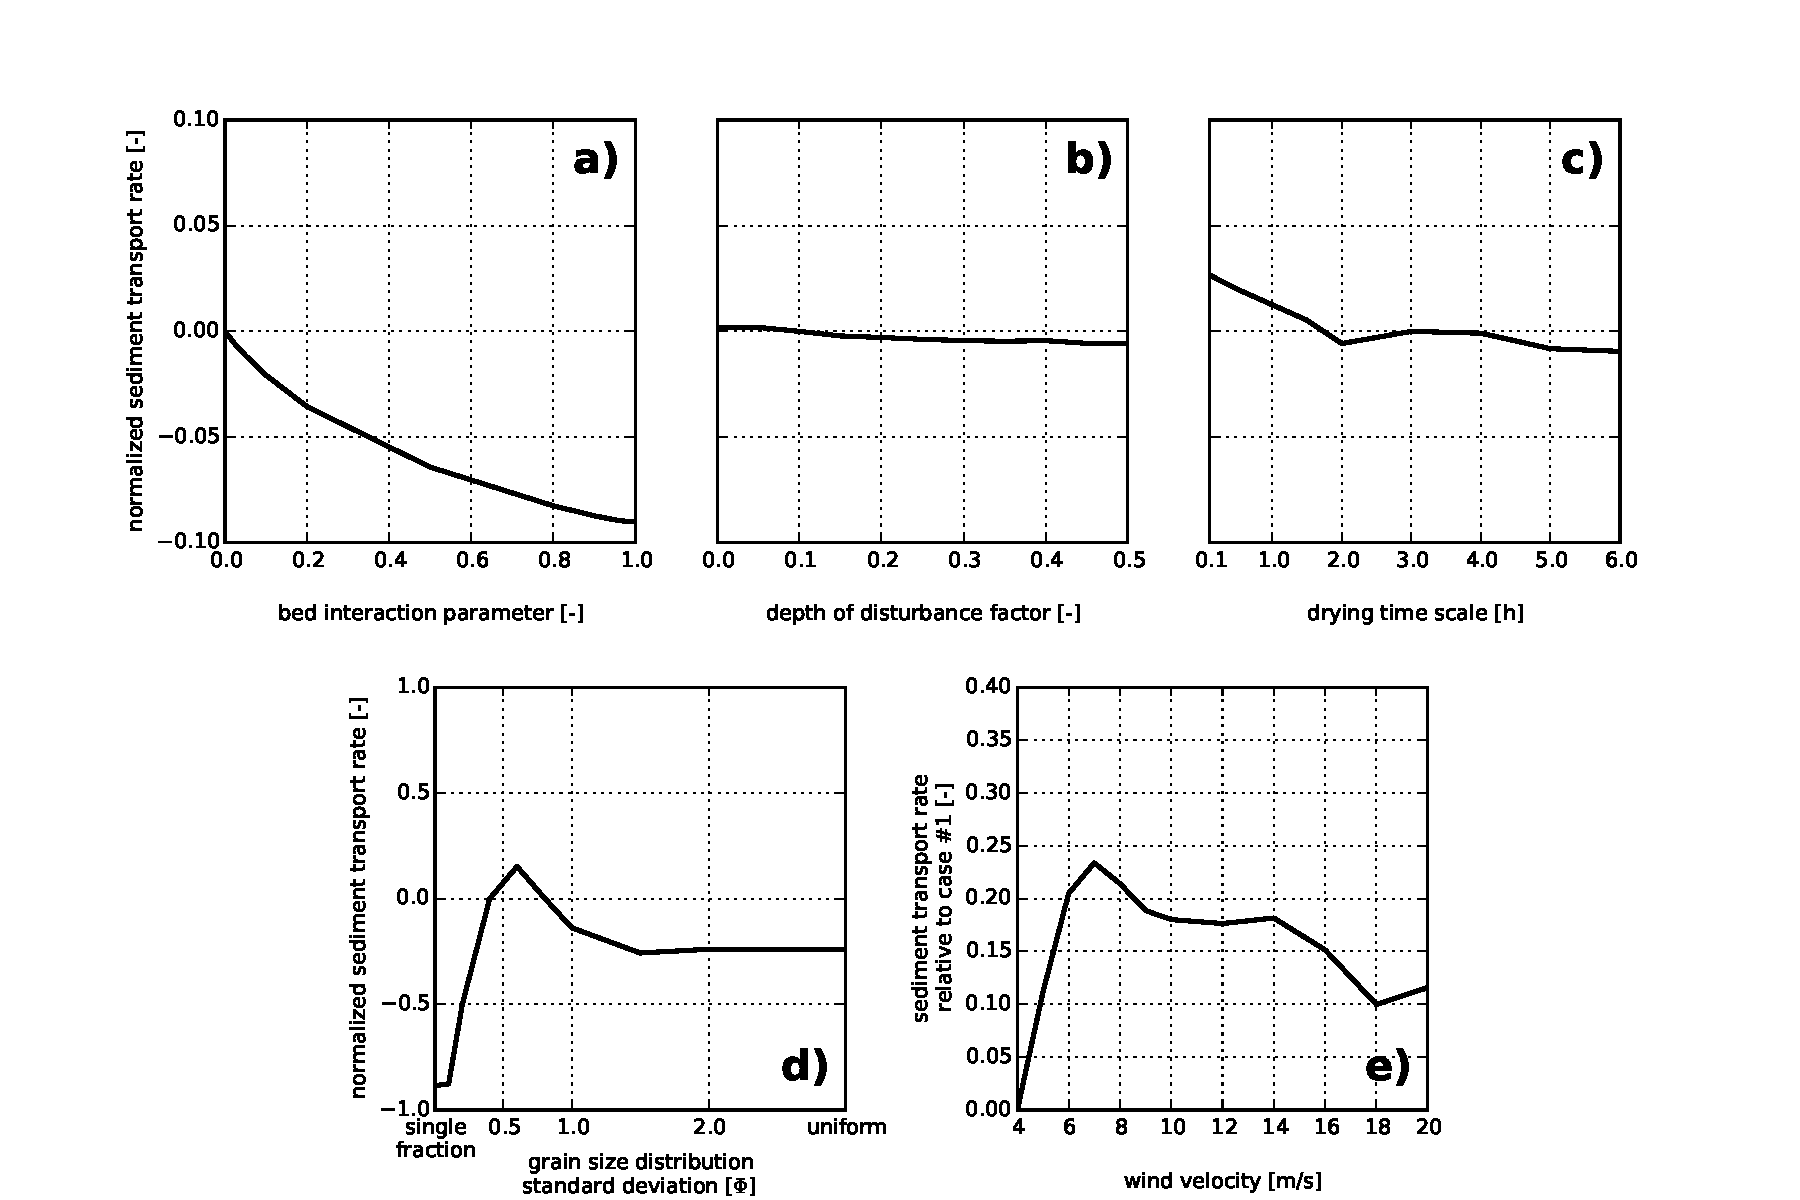
\includegraphics[width=\columnwidth]{../Figures/sensitivity_py}
  \caption{Sensitivity of the total normalized sediment transport with
    respect to case P3 for four newly introduced parameters and the
    wind velocity. The sensitivity of the wind velocity is expressed
    with respect to the transport rate in case P1.}
  \label{fig:sensitivity}
\end{figure}

The bed interaction parameter, the depth of disturbance factor and the
drying time scale affect the source area of aeolian sediment (Figure
\ref{fig:sensitivity}a, b and c). In absence of bed interaction all
sediment entrained in the intertidal beach area is being transported
to the downwind end of the domain unhindered. In contrast, in the
presence of bed interaction sediment from the intertidal beach area
may be trapped in the beach armor layer that is being developed in the
dry beach area during the simulation. Consequently, the total sediment
transport reduces with increasing bed interaction. The bed interaction
parameter parameterizes the exchange between sediment fractions, which
is an aspect of saltation that is still poorly understood.  In
particular situations with a large spatial variability in bed surface
properties the bed interaction parameter is expected to show a more
significant sensitivity \citep[e.g.][]{Dong2004b}. Therefore
calibration of the bed interaction parameter is necessary in such
situations.

The depth of disturbance factor shows no significant sensitivity as
aeolian sediment supply from the intertidal beach is concentrated
close to the water line where wave heights are negligible. Lower parts
of the intertidal beach are continuously too moist for sediment to be
entrained. The sensitivity to the depth of disturbance factor
increases with decreasing drying time scale, but typically only for
values smaller than 0.5 m.  The sensitivity to the drying time scale
shows that for time scales larger than several hours the intertidal
beach is continuously too moist for sediment to be entrained. For
small drying time scales the intertidal beach supplies aeolian
sediment that contains relatively many fines, resulting in a slight
increase in total sediment transport.

% The depth of disturbance factor and the drying time scale show a
% significant sensitivity (Figure \ref{fig:sensitivity}b and c). These
% parameters govern the sediment availability in the intertidal beach
% zone, which is ultimately the prime sediment source in case P3. In
% general, the large sensitivity to these parameters is expected in
% simulations where both beach armoring and tides play a role. Both
% parameters are related to peripheral processes in the presented
% model that are currently implemented using simplified
% formulations. Given the large sensitivity it seems advisable to
% further validate and possibly improve the implementation of these
% processes, which is considered outside the scope of this paper.
%
% For extreme values of both the depth of disturbance factor and the
% infiltration time scale the sensitivity reduces significantly. The
% sensitivity reduces for large depths
% ($f_{\Delta z_{\mathrm{d}}} > 0.5$) as the amount of fines becomes
% larger than the cumulative sediment transport capacity during the
% simulation.  The infiltration time scale shows two extreme
% situations in which the soil either does not dry out within a tidal
% cycle ($T_{dry} > 20$ h) or dries out instantly ($T_{dry} < 1$ h).

From the sensitivity of the grain size distribution width, represented
by the grain size distribution standard deviation and strictly
speaking not a model parameter, it can be concluded that the
introduction of multiple sediment fractions has a significant impact
on the sediment transport rate (Figure \ref{fig:sensitivity}d).
However, for poorly sorted sediments the sensitivity of the model to
the distribution width is limited. Beyond a standard deviation of
$\sigma_{\Phi} = 1.5$ the development of the sediment rate is similar
to the transport rate with a uniform distribution.

% The lowest sensitivity of the model is found for the bed interaction
% parameter (Figure \ref{fig:sensitivity}a). The bed interaction
% parameter parameterizes the exchange between sediment fractions,
% which is an aspect of saltation that is still poorly
% understood. Therefore calibration of the bed interaction parameter
% is necessary. A low sensitivity is beneficial as it reduces the
% importance of calibration. However, in particular situations with a
% large spatial variability in bed surface properties the bed
% interaction parameter is expected to show a more significant
% sensitivity \citep[e.g.][]{Dong2004b}.

The rate of armoring depends on the presence of non-erodible sediment
fractions. Whether a sediment fraction is erodible depends on the wind
transport capacity. Therefore the rate of armoring and consequently
the instantaneous sediment availability depends on the wind
velocity. Figure \ref{fig:sensitivity}e depicts the sediment transport
rate in case P3 with respect to the almost constant transport rate in
case P1 for different wind velocities. For low wind velocities all
shell fractions can contribute to the establishment of a beach armor
layer, but the beach armor layer develops slowly as the winnowing of
fines is dependent on the entrainment rate. For high wind velocities
even shell fragments may be mobilized, but the beach armor layer
consisting of larger shells is developed quickly. Consequently, the
reduction of sediment transport is present over all wind velocities
and 83\% on average.

% For low wind velocities all shell fractions can contribute to the
% establishment of a beach armor layer and consequently the sediment
% transport in case P3 is negligible compared to the transport rate in
% case P1. For high wind velocities, even shell fractions are
% mobilized and the importance of the beach armor layer
% reduces. Consequently, the sediment transport rates in case P3
% approach those of case P1 for high wind velocities.

\section{Discussion}

Process-based simulation of bed surface properties and sediment supply
provides an alternative for complex spatiotemporal
parameterizations. Nevertheless, process-based simulation itself
requires parameterization, calibration and validation. These
parameterizations are generally less complex as they describe static
properties rather than spatiotemporal varying processes.

\subsection{Parameterization}

Compared to existing models for availability-limited aeolian sediment
transport the need for complex parameterization has been reduced in
the presented model. The adoption of the advection model of
\citet{deVries2014a} makes parameterization of spatiotemporal
variations in the shear velocity threshold, like attempted by
\citet{Nickling1995}, \citet{Dong2004b} and others, unnecessary. In
addition, process-based simulation of bed surface properties makes
parameterization of the inherently time-varying sediment availability
$m_{\mathrm{a}}$ unnecessary. Existing parameterizations for the shear
velocity threshold under influence of moisture, vegetation, sediment
sorting and other bed surface properties are still valid for the
instantaneous shear velocity threshold.
% The proposed model provides a natural distinction between the fluid
% and impact threshold as these are related to the sediment
% availability and transport capacity that are both explicitly
% defined.

Despite the efforts to minimize complex parameterizations that are
difficult to generalize, the model also introduces new
parameterizations that are specifically related to the process-based
simulation of sediment availability, i.e. the bed interaction
parameter, depth of disturbance and soil drying time scale. The depth
of disturbance and soil drying time scale could easily be replaced by
process-based simulation as there is thorough knowledge on near-shore
morphodynamics and beach hydrology. Moreover, the presented model
framework allows for spatiotemporal variations of parameters that are
known not to be constant (e.g. $z'$). However, these considerations
are outside the scope of this paper and will be part of future
research.

\subsection{Calibration}

The calibration of the parameters involved in process-based simulation
of sediment availability is a relatively new field of research. In
this paper a pragmatic approach to calibration of these parameters is
adopted, but there are various opportunities for improvement. For
example, the depth of disturbance is used to approximate the mixing of
the intertidal beach surface by waves. \citet{Masselink2007} shows how
the depth of disturbance can be determined based on a linear relation
with the local wave height. The mixing of the intertidal beach surface
is particularly important as it breaks beach armoring. The depth of
disturbance does not provide any information about how the bed is
disturbed, just over which depth. Moreover, aspects like marine
deposits and shell buoyancy also affect the sediment availability in
the intertidal beach area. \citet{Gallagher2011} presented detailed
measurements of spatiotemporal variations in the bed surface grain
size at Truc Vert, France. The intertidal beach appears to be
consistently finer than the upper beach. The measurements are obtained
using macrophotography \citep{Buscombe2010} ensuring that the
measurements solely involve the beach surface. These type of
measurements may provide a much more detailed calibration of the
hydraulic mixing simulated in the model, although it might be
questioned if such detailed hydraulic calibration is still within the
scope of an aeolian sediment transport model. Alternatively, the
calibration of the hydraulic mixing could be left to dedicated
near-shore models \citep[e.g. XBeach;][]{Roelvink2009,Reniers2013} and
online model coupling could be used to incorporate detailed near-shore
hydro- and morphodynamics in the proposed aeolian modeling framework.

Similarly, an exponential decay function with a constant drying
time scale is currently used to approximate the influence of the
hydrological process of infiltration. The exponential decay is a
simplified approach that was adopted after it appeared to be a
reasonable approximation of numerical model results obtained with the
HYDRUS model \citep{Simunek1998} that simulates the soil moisture
contents in the unsaturated zone following
\citet{Genuchten1978}. Detailed measurements for calibration of the
instantaneous soil moisture can be obtained relatively easy using
either in-situ or remote infra-red or microwave measurements
\citep[e.g.][]{Edwards2013, Hoonhout2014}. Again, it might be
questioned if the amount of detail involved in using these kind of
data for estimates of the bed surface moisture is still within the
scope of an aeolian sediment transport model.

In contrast to the depth of disturbance and the drying rate, the bed
interaction parameter has little relation with existing literature. In
essence, the bed interaction parameter describes the exchange of
momentum between grain size fractions along the fetch
distance. Specifically it describes whether impacting grains eject
other grains from the bed or that they are rebounded due to fully
elastic collisions with large, non-erodible elements. A low value for
the bed interaction parameter would indicate a large number of
rebounding grains, while a high value would indicate a low number of
rebounding grains. Typically, the number of rebounded grains increases
with an increasing number of non-erodible, large elements in the
bed. Consequently, the bed interaction parameter is not uniform over
the fractions. Moreover, due to beach armoring the bed interaction is
neither constant over time nor in space. In this paper the bed
interaction parameter is pragmatically assumed to be uniform and
constant since no basis for differentiation of the parameter is
currently available. Thorough calibration of the bed interaction
parameter would require detailed, spatiotemporal measurements of grain
size distributions in the bed and the saltation cascade. It would
require a series of sediment traps along the fetch that are regularly
emptied and sieved as to determine the change of the grain size
distribution in the saltation cascade in space and over
time. Concurrently the grain size distribution at the bed surface over
the entire fetch needs to be monitored without disturbing the bed
significantly. In a laboratory environment the change in grain size
distribution could be monitored using sediment that is colored per
fraction. Visual observation of the change in coloring then provides
insight in the change in grain size distribution. However, the
experiment should be performed at such scale that the trapping of
sediment by upwind traps does not significantly influence the
saltation cascade downwind over the period that the armor layer
develops.

\subsection{Validation}

Validation of the proposed model is ongoing. Initially, validation
will be focused on gross sediment transport rates in
availability-limited systems. Few holistic measurements are available
that monitor both the spatiotemporal variations in the sediment
transport rate and the availability-limiting factors like moisture
content and beach armoring concurrently
\citep[e.g.][]{DelgadoFernandez2012, Hoonhout2013}. Sites with
detailed and frequent topographic measurements and hydrodynamic
boundary conditions available can be found worldwide. These sites
would be a good starting point for assessing the performance of the
model compared to existing models. Using simplified, but generic
descriptions of the hydraulic mixing and drying rate the model should
already provide time series of aeolian sediment transport that adhere
much better to the true nature of aeolian sediment transport events
than existing models. \citet{DelgadoFernandez2011} and
\citet{deVries2014b} already indicated that the true nature of these
events is not solely related to wind velocity and direction, but also
to surges, seasons, spring/neap cycles, rain showers and other events
that influence sediment availability. The variations in aeolian
sediment transport due to these event-driven changes in sediment
availability are not well captured by models that rely solely on the
wind transport capacity. The model has added value if it improves the
prediction of transport rates under such circumstances.

%\subsection{Model coupling}
%
%Apart from calibration and validation of the proposed model it is
%worth examining how this model and the related knowledge on
%availability-limited systems can be fitted in the broader
%understanding of coastal dynamics. As illustrated in this paper,
%aeolian sediment transport cannot be seen independently of near-shore
%hydrodynamics and related sediment transport, hydrology and probably
%also meteorology. Combining all these processes in a single sediment
%transport model would be cumbersome. Most prominently it would involve
%the combination of processes at time scales from seconds to
%years. Mathematically this would be challenging in terms of optimal
%numerical schemes and related time steps. Practically, as excellent
%models that simulate these processes already exist, it would require
%close and permanent collaboration between disciplines which might not
%be feasible on the long term.
%
%Instead, existing models could be seen as building blocks in a larger
%modeling framework for coastal sediment transport. This philosophy is
%the basis of online model coupling techniques, like the Earth System
%Modeling Framework \citep[ESMF;][]{Hill2004} and the Basic Model
%Interface \citep[BMI;][]{Peckham2013}. Online model coupling allows
%model cores to communicate with each other during the simulation. A
%near-shore hydrodynamic model like XBeach \citep{Roelvink2009} can
%therefore supply detailed descriptions of the water level, wave height
%and near-shore morphodynamics like onshore bar migration
%\citep{Cohn2015} to an aeolian sediment transport model. A
%hydrological model like HYDRUS \citep{Simunek1998} might be used to
%estimate instantaneous bed surface moisture contents. Even the wind
%field might be borrowed from a model like the highly efficient Coastal
%Dune Model \citep[CDM;][]{Duran2013}. In conclusion, online model
%coupling provides an elegant alternative to the few simplified
%implementations currently used in the proposed model.

\section{Conclusions}

The \textsc{AeoLiS} model presented in this paper is the first aeolian
sediment transport model that simulates spatiotemporal variations in
bed surface properties and sediment availability. Simulation of
sediment availability is necessary as sediment availability cannot be
determined a-priori due to its recurrence relation with sediment
transport. The presented model approach is a generalization of
existing modeling concepts for aeolian sediment transport that include
the influence of bed surface properties and limitations in sediment
availability, like the shear velocity threshold and critical fetch,
and is compatible with these concepts. The model uses an advection
scheme following \citet{deVries2014a} and a bed composition module
that discretizes the bed in horizontal grid cells and vertical bed
layers to account for spatial variations in bed surface
properties. Temporal variations in sediment availability are not
parameterized, but simulated using the bed composition module. The
simulation of sediment availability reduces the need for complex
spatiotemporal parameterizations and consequently calibration. In this
paper the influence of sediment sorting and beach armoring and the
reversed process of hydraulic mixing on aeolian sediment transport are
illustrated using four prototype cases. The model can reproduce
patterns in aeolian sediment availability and transport as observed in
wind tunnel experiments that involve spatiotemporal variations in bed
surface properties \citep{Nickling1995, Dong2004b}. Further, the model
provides a generic framework to incorporate additional spatiotemporal
varying processes that either influence sediment availability or the
wind transport capacity with a minimum of parameterization. The
framework allows relatively straightforward implementation of the
effects of infiltration, evaporation, vegetation, buildings, and
morphological feedback with the wind.
%Also, the model allows for
%online coupling with other models that accurately describe related
%physics that are currently parameterized like hydrodynamics, hydrology
%and meteorology.

\vspace{.5cm}

\noindent From this paper the following conclusions can be drawn:

\begin{enumerate}
\item A model for aeolian sediment transport was presented that
  simulates the processes of sediment sorting and beach armoring, the
  reversed process of hydraulic mixing, interaction between sediment
  fractions in the air with sediment fractions in the bed and thereby
  the influence of spatiotemporal variations in sediment availability;
\item The model can be seen as a generalization of existing approaches
  to incorporate limitations in sediment availability and the wind
  transport capacity in aeolian transport estimates and is compatible
  with approaches based on either shear velocity thresholds or
  critical fetch;
\item The process of beach armoring can be a
  governing factor in aeolian sediment transport modeling and may
  reduce the estimated transport rates significantly and up to 95.0\% in
  the presented prototype cases;
\item The model can reproduce typical patterns in aeolian sediment
  transport with spatiotemporal variations in sediment availability
  obtained from measurements from the unrelated wind tunnel
  experiments described in \citet{Nickling1995} and \citet{Dong2004b},
  with a minimum parameterization and calibration.
\end{enumerate}

%%% Local Variables:
%%% mode: latex
%%% TeX-master: "thesis"
%%% End:
